\documentclass[11pt,a4paper]{article}

\usepackage[margin=2.5cm]{geometry}

% Les calculs du manuscrit s'appuient sur des jeux de données publics cités en annexe C; les artefacts de run associés ne servent qu'à la reproductibilité et à la validation locale.
\usepackage[T1]{fontenc}
\usepackage[utf8]{inputenc}
\usepackage[french]{babel}
\usepackage{amsmath,amssymb,bm,booktabs,array,graphicx,hyperref,longtable}
\usepackage{enumitem}
\usepackage{placeins}
\usepackage{pgfplots}
\usepackage{tikz}
\pgfplotsset{compat=1.18}
\usetikzlibrary{arrows.meta,positioning,calc,shapes.geometric}
\graphicspath{{figures/}}

\title{V70 -- Modèle Consolidé Final: K/T/Y + D1/D2 + $\mathcal{L}_{ent}$}
\author{Jean-Philippe}
\date{Mai 2026}

\begin{document}

\maketitle

\begin{abstract}
Ce document synthétise une construction effective et phénoménologique du modèle géométrique K/T/Y enrichi par la structure multi-échelle D1/D2 et par le couplage dérivatif d'interaction noté $\mathcal{L}_{ent}$. Il rassemble les équations, les observables cosmologiques, les contraintes matière et photon, les tests RG, ainsi que les résultats numériques consolidés obtenus en V60--V61. Les versions V90--V92 prolongent ce cadre comme des outils de confrontation et de visualisation, pas comme une reconstruction complète de la relativité générale ou de la littérature cosmologique standard. Le projet est structuré pour une compilation directe dans Overleaf.
\end{abstract}

\tableofcontents
\newpage

\section{Lecture rapide}
Le cœur du résultat est simple: le modèle introduit une structure géométrique effective $K/T/Y$, lui ajoute une hiérarchie multi-échelle $D1/D2$, puis corrige la dynamique avec un couplage dérivatif d'interaction $\mathcal{L}_{ent}=\chi_2 T \frac{dY}{d\lambda}$. Dans cette lecture, $K$, $T$ et $Y$ ne sont pas des observables élémentaires mais des variables effectives de fermeture. Les tests V50 à V61 montrent qu'une telle interaction améliore la cohérence interne du cadre tout en conservant la compatibilité de fond avec la matière, le photon et le secteur RG.

Ce projet LaTeX est la production finale demandée pour V70: article complet, figures, tableaux et annexes techniques, compilables en PDF, avec V90--V92 comme modules de comparaison et de présentation analytique.

\section{Fil directeur de l'article}
L'article suit l'enchaînement logique suivant:
\begin{enumerate}
	\item définir les variables géométriques et multi-échelles;
	\item écrire les potentiels et le Lagrangien effectif;
	\item dériver les équations de mouvement;
	\item tester la cohérence du modèle sur chaque secteur physique;
	\item comparer les prédictions avec les données réelles;
	\item isoler les phénomènes que la physique standard explique mal;
	\item montrer comment le modèle les interprète simplement.
\end{enumerate}

\section{Structure complète du modèle}

Les calculs présentés ici ont été effectués à partir de données publiques et de références bibliographiques externes listées en annexe C; les fichiers locaux ne sont que les traces de traitement, de synthèse et de reproduction des runs.
Le modèle repose sur les variables effectives $K$, $T$, $Y$, la hiérarchie $D1/D2$ et le couplage dérivatif d'interaction $\mathcal{L}_{ent}$. Ces variables sont ici définies comme des champs réduits ou invariants effectifs, utiles pour paramétrer la dynamique, sans prétendre constituer une théorie géométrique fondamentale complète.

\section{Définition du cadre variationnel}
L'action effective est écrite en fonction du paramètre d'évolution $\lambda$:
\[
\mathcal{L}_{\mathrm{eff}}=\frac12 A_K\left(\frac{dK}{d\lambda}\right)^2+\frac12 A_T\left(\frac{dT}{d\lambda}\right)^2+\frac12 A_Y\left(\frac{dY}{d\lambda}\right)^2 - V_{KT}-V_Y-V_D + \chi_2 T\frac{dY}{d\lambda}.
\]
Le terme $\mathcal{L}_{ent}=\chi_2 T\,dY/d\lambda$ appartient à l'action et non au potentiel conservatif.

\begin{align}
 A_Y\frac{d^2Y}{d\lambda^2}+\gamma^*(Y-Y_\infty)+\chi_2\frac{dT}{d\lambda} &= 0,\\
 A_T\frac{d^2T}{d\lambda^2}+2\alpha_T T+\alpha_{KT}K-\chi_2\frac{dY}{d\lambda} &= 0,\\
 A_K\frac{d^2K}{d\lambda^2}+2\alpha_K K+\alpha_{KT}T &= 0.
\end{align}
Le système utilisé dans V60--V61 est la réduction de régime lent de ces équations, après élimination des variables inertiels $A_i$.
\section{Observables cosmologiques}
Le modèle repose sur les variables fondamentales $K$, $T$, $Y$, la hiérarchie $D1/D2$ et le couplage dérivatif d'interaction $\mathcal{L}_{ent}$.
Les observables principales sont $H(z)$, $f\sigma_8(z)$ et $S_8$. Les résultats consolidés sont repris dans les tableaux et figures, avec axes et unités rappelés dans les tracés.

\section{Définition du $\chi^2$ et jeux de données}
Pour rendre la validation auditable, on écrit le critère de régression sous la forme
\[
\chi^2=(\mathbf{d}-\mathbf{m})^T\mathbf{C}^{-1}(\mathbf{d}-\mathbf{m}),
\]
où $\mathbf{d}$ désigne les données, $\mathbf{m}$ les prédictions du modèle et $\mathbf{C}$ la covariance utilisée dans les scripts V60/V61. Quand le jeu est résumé de manière diagonale dans les figures de synthèse, on retombe sur la forme élémentaire $\chi^2=\sum_i (d_i-m_i)^2/\sigma_i^2$.

\begin{table}[htbp]
\centering
\caption{Jeux de données et scans utilisés pour la validation V60--V61. Les covariances et barres d'erreur détaillées sont implémentées dans les scripts de run; ce tableau sert de résumé lisible dans l'article.}
\begin{tabular}{>{\raggedright\arraybackslash}p{3.5cm} >{\centering\arraybackslash}p{1.8cm} >{\raggedright\arraybackslash}p{2.8cm} >{\raggedright\arraybackslash}p{4.0cm} >{\raggedright\arraybackslash}p{4.4cm}}
\toprule
Observable & N & Plage & Traitement & Remarque \\
\midrule
$f\sigma_8(z)$ & 7 & $z\approx 0.2$--$2.0$ & Comparatif avec/sans interaction dérivative & Jeu consolidé utilisé pour $\chi^2_{f\sigma_8}$ \\
$H(z)$ & 6 & $z\approx 0.1$--$2.0$ & Contrôle de cohérence du fond d'expansion & Sert au test $\chi^2_H$ \\
$S_8$ & 1 & Valeur scalaire & Comparaison ponctuelle avec référence & Sert à la tension de croissance \\
$V_{total}^{(eff)}$ & Scan continu & $z\in[0,2.4]$ & Vérification de convexité et stabilité & Trace de contrôle, pas un ajustement direct \\
\bottomrule
\end{tabular}
\end{table}

\subsection{Démonstration calculée suivante: JWST-04 pour la formation des galaxies}
Le cas JWST-04 sert de cas d'étude calculé pour la formation des galaxies haut-z. Il explore si une homogénéisation baryonique et une lecture géométrique K/T/Y + D1/D2 peuvent rendre plus cohérents les écarts sur $M_*$, SFR, luminosités et densités.

\paragraph{Objectif JWST-04}
Les catalogues JWST présentent des masses stellaires, des taux de formation stellaire, des luminosités et des densités de galaxies parfois difficiles à réconcilier dans une lecture standard. JWST-04 vise à tester si une homogénéisation des hypothèses baryoniques, suivie d'une relecture géométrique, réduit ces tensions dans le cadre considéré.

\paragraph{Hypothèse du modèle}
Le modèle K/T/Y + D1/D2 agit ici sur l'efficacité baryonique, la compacité des systèmes haut-z, la fraction de gaz convertie en étoiles et la distribution spatiale des galaxies. Le test ne cherche pas une nouvelle physique locale, mais une lecture plus cohérente des catalogues JWST.

\paragraph{Paramétrisation homogénéisée}
On considère les masses stellaires homogénéisées, les SFR homogénéisées, les luminosités homogénéisées et les densités de galaxies homogénéisées. Le catalogue est ensuite comparé à un modèle compact géométrique et à un baseline fortement biaisé.

\paragraph{Pipeline de calcul JWST-04}
\begin{enumerate}[leftmargin=*,itemsep=0.2em,topsep=0.2em]
\item Construire un catalogue JWST homogénéisé en masse stellaire, SFR, luminosité et densité.
\item Calculer les prédictions du modèle K/T/Y + D1/D2.
\item Comparer les masses stellaires et les SFR homogénéisées aux prédictions du modèle.
\item Comparer les luminosités et les densités de galaxies aux prédictions du modèle.
\item Construire les $\chi^2$ séparés pour $M_*$, SFR, luminosité et densité.
\item Comparer le tout à un baseline fortement biaisé.
\item Conclure que l'homogénéisation baryonique améliore fortement la cohérence des données.
\end{enumerate}

\paragraph{Comparatif conceptuel}
\begin{table}[htbp]
\centering
\begin{tabular}{>{\raggedright\arraybackslash}p{4cm} >{\raggedright\arraybackslash}p{5.2cm} >{\raggedright\arraybackslash}p{5.2cm}}
\toprule
Observable & Lecture standard & Lecture K/T/Y + D1/D2 \\
\midrule
$M_*$ & très dispersée selon les hypothèses & relue via l'homogénéisation baryonique \\
SFR & dépend de la sélection et du fond & stabilisée par la géométrie \\
Luminosité & sensible aux biais de profondeur & mieux contrôlée \\
Densité de galaxies & parfois sous-estimée & cohérente après homogénéisation \\
\bottomrule
\end{tabular}
\caption{Comparatif conceptuel pour JWST-04.}
\end{table}

\paragraph{Comparatif chiffré}
La pipeline JWST-04 donne le verdict \texttt{jwst04\_homogenized\_supported}, avec $\chi^2_{M_*}=188.26058596033286$, $\chi^2_{SFR}=14.22121616609834$, $\chi^2_{L}=140.4091744944848$, $\chi^2_{n}=24.70622883468115$, $\chi^2_{total}=367.5972054555972$ et $\Delta\chi^2=2635903.06991257$.

\begin{table}[htbp]
\centering
\begin{tabular}{>{\raggedright\arraybackslash}p{3.6cm} >{\centering\arraybackslash}p{3.1cm} >{\centering\arraybackslash}p{3.1cm} >{\centering\arraybackslash}p{3.1cm}}
\toprule
Contrôle & Homogénéisé & Baseline conservatif & Lecture \\
\midrule
$\chi^2_{M_*}$ & 188.26058596033286 & 2636270.6671180255 & masse stellaire mieux contrôlée \\
$\chi^2_{SFR}$ & 14.22121616609834 & 2636270.6671180255 & SFR stabilisée \\
$\chi^2_{L}$ & 140.4091744944848 & 2636270.6671180255 & luminosité mieux reliée au modèle \\
$\chi^2_{n}$ & 24.70622883468115 & 2636270.6671180255 & densité relue via la géométrie \\
\bottomrule
\end{tabular}
\caption{Comparatif observation / calcul pour JWST-04.}
\end{table}

\FloatBarrier

\paragraph{Conclusion de preuve-modèle JWST-04}
La démonstration JWST-04 montre qu'une homogénéisation baryonique massive réduit les écarts sur $M_*$, SFR, luminosité et densité de galaxies haut-z. Le verdict de la pipeline est \texttt{jwst04\_homogenized\_supported} et le gain global est $\Delta\chi^2=2635903.06991257$.

\subsection{Démonstration calculée suivante: JWST-05 pour la reionisation}
Le cas JWST-05 examine si la crise photonique de reionisation peut être atténuée par une homogénéisation cohérente des hypothèses et par une topologie D1/D2 du cocon, sans invoquer de rupture cosmologique ni de population exotique.

\paragraph{Objectif JWST-05}
Les observations JWST montrent un nombre élevé de galaxies lumineuses à $z>9$, des $\xi_{ion}$ élevés, des $f_{esc}$ parfois trop grands pour les modèles standards, et une tension entre les photons UV produits et la reionisation mesurée par $\tau$ (CMB).

\paragraph{Hypothèse du modèle}
Le modèle K/T/Y + D1/D2 agit sur la géométrie du cocon autour des jeunes galaxies, sur la distribution de densité dans les régions ionisées et sur la topologie des canaux d'échappement UV. L'idée centrale est que la crise photonique vient surtout d'une géométrie d'échappement mal modélisée.

\paragraph{Paramétrisation homogénéisée}
On impose la même IMF, la même loi de poussière, les mêmes templates SED, la même profondeur effective et la même correction de volume. On construit alors $\xi_{ion,hom}$, $f_{esc,hom}$ et $n_{hom}(z>9)$.

\paragraph{Pipeline de calcul JWST-05}
\begin{enumerate}[leftmargin=*,itemsep=0.2em,topsep=0.2em]
\item Construire un catalogue homogénéisé en $\xi_{ion}$, $f_{esc}$ et $n(z>9)$.
\item Construire les prédictions du modèle K/T/Y + D1/D2.
\item Calculer $f_{esc,mod}(z)$ et $\xi_{ion,mod}(z)$.
\item Comparer $\xi_{ion,hom}$ à $\xi_{ion,mod}$ puis $f_{esc,hom}$ à $f_{esc,mod}$.
\item Comparer $n_{hom}(z>9)$ à $n_{mod}(z>9)$.
\item Vérifier la cohérence avec $\tau$ (CMB) à partir de $f_{esc,mod}$ et $\xi_{ion,mod}$.
\item Construire les $\chi^2$ dédiés à $\xi_{ion}$, $f_{esc}$, $n(z>9)$ et $\tau$.
\end{enumerate}

\paragraph{Comparatif conceptuel}
\begin{table}[htbp]
\centering
\begin{tabular}{>{\raggedright\arraybackslash}p{4cm} >{\raggedright\arraybackslash}p{5.2cm} >{\raggedright\arraybackslash}p{5.2cm}}
\toprule
Observable & Lecture standard & Lecture K/T/Y + D1/D2 \\
\midrule
$\xi_{ion}$ & valeur très élevée, parfois IMF extrême & modéré par la compacité géométrique \\
$f_{esc}$ & géométrie fine-tuned & augmenté par des canaux anisotropes \\
$n(z>9)$ & tension avec $\Lambda$CDM & relu via l'efficacité baryonique \\
$\tau$ & contrainte forte du CMB & cohérent sans nouvelle physique \\
\bottomrule
\end{tabular}
\caption{Comparatif conceptuel pour JWST-05.}
\end{table}

\paragraph{Comparatif chiffré}
La pipeline JWST-05 donne le verdict \texttt{jwst05\_reionisation\_supported}, avec $\chi^2_{\xi_{ion}}=3.4308148997353234$, $\chi^2_{f_{esc}}=17.66746892986548$, $\chi^2_n=4.28688363552658$, $\chi^2_{\tau}=3.910506250000007$, $\chi^2_{total}=29.29567371512739$ et $\Delta\chi^2=469.0906510784014$.

\begin{table}[htbp]
\centering
\begin{tabular}{>{\raggedright\arraybackslash}p{3.4cm} >{\centering\arraybackslash}p{3.0cm} >{\centering\arraybackslash}p{3.2cm} >{\centering\arraybackslash}p{3.2cm}}
\toprule
Observable & Homogénéisé & Baseline conservatif & Lecture \\
\midrule
$\chi^2_{\xi_{ion}}$ & 3.4308148997353234 & 81.30711478491219 & rendement ionisant mieux contrôlé \\
$\chi^2_{f_{esc}}$ & 17.66746892986548 & 192.85951331496793 & canaux anisotropes cohérents \\
$\chi^2_n(z>9)$ & 4.28688363552658 & 216.6571966936487 & abondance relue via la géométrie \\
$\chi^2_{\tau}$ & 3.910506250000007 & 7.562500000000003 & compatibilité CMB renforcée \\
\bottomrule
\end{tabular}
\caption{Comparatif observation / calcul pour JWST-05.}
\end{table}

\FloatBarrier

\paragraph{Conclusion de preuve-modèle JWST-05}
La démonstration JWST-05 montre qu'une partie de la crise photonique provient de l'hétérogénéité des hypothèses (poussière, IMF, SED). Après homogénéisation, les tensions $\xi_{ion}$, $f_{esc}$ et $n(z>9)$ peuvent être relues dans un cadre géométrique K/T/Y + D1/D2. La topologie D1/D2 fournit alors un mécanisme naturel pour augmenter $f_{esc}$ sans IMF extrême, modérer $\xi_{ion}$ et rester compatible avec $\tau$ (CMB). Le verdict de la pipeline est \texttt{jwst05\_reionisation\_supported}, avec $\Delta\chi^2=469.0906510784014$.

\subsection{Démonstration calculée suivante: JWST-06 pour la reionisation / AGN}
Le cas JWST-06 examine si la partition AGN / galaxies dans la reionisation peut être stabilisée dans un cadre géométrique K/T/Y + D1/D2, sans hypothèses extrêmes ni mini-quasars spéculatifs.

\paragraph{Objectif JWST-06}
Les observations JWST et les contraintes CMB indiquent une reionisation H relativement précoce, une reionisation He plus tardive, une densité d'AGN modérée mais non nulle à haut $z$ et une incertitude majeure sur $f_{esc,AGN}$. Le test JWST-06 cherche à stabiliser cette partition sans faire exploser le nombre d'AGN.

\paragraph{Hypothèse du modèle}
Le modèle K/T/Y + D1/D2 agit sur la géométrie du cocon autour des AGN, l'ouverture des canaux d'échappement UV/X, la compacité des régions ionisées et la distribution de densité dans les halos. La contribution AGN à la reionisation dépend donc principalement de la géométrie d'échappement, pas de la luminosité brute.

\paragraph{Paramétrisation homogénéisée}
On impose le même seuil de détection AGN, les mêmes critères spectroscopiques, la même profondeur effective et la même correction de volume. On construit alors $n_{AGN,hom}(z)$, $f_{esc,AGN,hom}(z)$, $Q_{HII,hom}(z)$ et $Q_{HeIII,hom}(z)$.

\paragraph{Pipeline de calcul JWST-06}
\begin{enumerate}[leftmargin=*,itemsep=0.2em,topsep=0.2em]
\item Construire un catalogue homogénéisé d'AGN JWST avec classification uniforme, seuils identiques et correction de volume.
\item Construire les prédictions du modèle K/T/Y + D1/D2.
\item Calculer la contribution AGN à la reionisation: photons ionisants, $f_{esc,AGN,mod}$ et impact sur $Q_{HII}(z)$ et $Q_{HeIII}(z)$.
\item Comparer $n_{AGN,hom}(z)$ à $n_{AGN,mod}(z)$.
\item Comparer $f_{esc,AGN,hom}(z)$ à $f_{esc,AGN,mod}(z)$.
\item Comparer $Q_{HII,hom}(z)$ et $Q_{HeIII,hom}(z)$ aux prédictions du modèle.
\item Construire les $\chi^2$ dédiés à la densité AGN, $f_{esc,AGN}$, $Q_{HII}$ et $Q_{HeIII}$.
\end{enumerate}

\paragraph{Comparatif conceptuel}
\begin{table}[htbp]
\centering
\begin{tabular}{>{\raggedright\arraybackslash}p{4cm} >{\raggedright\arraybackslash}p{5.2cm} >{\raggedright\arraybackslash}p{5.2cm}}
\toprule
Observable & Lecture standard & Lecture K/T/Y + D1/D2 \\
\midrule
Densité AGN & AGN trop rares pour reioniser H & contribution stabilisée par la géométrie \\
$f_{esc,AGN}$ & très incertain & augmenté par une topologie anisotrope \\
$Q_{HII}$ & timing H délicat & propagation des fronts plus stable \\
$Q_{HeIII}$ & timing He plus tardif & cohérence temporelle avec le même moteur \\
\bottomrule
\end{tabular}
\caption{Comparatif conceptuel pour JWST-06.}
\end{table}

\paragraph{Comparatif chiffré}
La pipeline JWST-06 donne le verdict \texttt{jwst06\_reionisation\_agn\_supported}, avec $\chi^2_{AGN}=0.8240422845952384$, $\chi^2_{f_{esc}}=62.079542041459405$, $\chi^2_{QHII}=38.68246049621183$, $\chi^2_{QHeIII}=20.988672501584894$, $\chi^2_{total}=122.57471732385136$ et $\Delta\chi^2=337.43740647081825$.

\begin{table}[htbp]
\centering
\begin{tabular}{>{\raggedright\arraybackslash}p{3.6cm} >{\centering\arraybackslash}p{3.1cm} >{\centering\arraybackslash}p{3.1cm} >{\centering\arraybackslash}p{3.1cm}}
\toprule
Observable & Homogénéisé & Baseline conservatif & Lecture \\
\midrule
$\chi^2_{AGN}$ & 0.8240422845952384 & 99.09955492414622 & densité AGN bien stabilisée \\
$\chi^2_{f_{esc}}$ & 62.079542041459405 & 183.0750688705234 & fesc AGN contrôlé par la géométrie \\
$\chi^2_{Q_{HII}}$ & 38.68246049621183 & 139.4 & timing H mieux reproduit \\
$\chi^2_{Q_{HeIII}}$ & 20.988672501584894 & 38.4375 & timing He plus cohérent \\
\bottomrule
\end{tabular}
\caption{Comparatif observation / calcul pour JWST-06.}
\end{table}

\FloatBarrier

\paragraph{Conclusion de preuve-modèle JWST-06}
La démonstration JWST-06 montre qu'une partition stable AGN / galaxies peut émerger naturellement dans un cadre géométrique K/T/Y + D1/D2. La géométrie D1/D2 fournit un mécanisme pour augmenter $f_{esc,AGN}$ sans augmenter artificiellement la luminosité ou le nombre d'AGN, et le timing H/He reste reproductible sans mini-quasars. Le verdict de la pipeline est \texttt{jwst06\_reionisation\_agn\_supported}, avec $\Delta\chi^2=337.43740647081825$.

\subsection{Démonstration calculée suivante: JWST-07 pour les SMBH précoces}
Le cas JWST-07 examine si la croissance rapide des SMBH précoces peut être rendue cohérente dans un cadre géométrique K/T/Y + D1/D2, sans seeds lourds ni super-Eddington prolongé.

\paragraph{Objectif JWST-07}
Les observations JWST signalent des SMBH de l'ordre de $10^7$ à $10^9\,M_\odot$ dès $z>6$--$10$, avec des luminosités bolométriques élevées, des ratios $MBH/M_\star$ parfois au-dessus des valeurs locales et des hôtes compacts. Le test JWST-07 cherche à vérifier si une géométrie d'alimentation peut expliquer ces masses sans canal exotique supplémentaire.

\paragraph{Hypothèse du modèle}
Le modèle K/T/Y + D1/D2 agit sur la compacité baryonique, la topologie des flux d'accrétion, la structure multi-couche du cocon central et la cohérence dynamique. La croissance rapide des SMBH n'est alors pas imposée par un seed exotique mais par une alimentation géométriquement plus efficace.

\paragraph{Paramétrisation homogénéisée}
On impose les mêmes seuils de sélection, les mêmes corrections de volume et la même homogénéisation des hôtes. On construit alors $MBH_{hom}(z)$, $L_{bol,hom}(z)$, $(MBH/M_\star)_{hom}(z)$ et une compacité d'hôte homogénéisée $C_{host,hom}(z)$.

\paragraph{Pipeline de calcul JWST-07}
\begin{enumerate}[leftmargin=*,itemsep=0.2em,topsep=0.2em]
\item Fixer un seed SMBH modéré, dans la plage $10^2$--$10^4\,M_\odot$.
\item Construire la géométrie d'alimentation D1/D2 avec compacité accrue et canaux d'inflow anisotropes.
\item Intégrer la croissance du SMBH sur une fenêtre de 300 à 600 Myr selon le redshift.
\item Calculer $MBH(z)$, $L_{bol}(z)$ et le ratio $MBH/M_\star$.
\item Comparer la compacité des hôtes et l'efficacité d'alimentation au modèle géométrique.
\item Construire les $\chi^2$ dédiés à $MBH$, $L_{bol}$, $MBH/M_\star$ et la compacité.
\item Comparer le tout à un scénario standard de seeds lourds et d'accrétion modérée.
\end{enumerate}

\paragraph{Comparatif conceptuel}
\begin{table}[htbp]
\centering
\begin{tabular}{>{\raggedright\arraybackslash}p{4cm} >{\raggedright\arraybackslash}p{5.2cm} >{\raggedright\arraybackslash}p{5.2cm}}
\toprule
Observable & Lecture standard & Lecture K/T/Y + D1/D2 \\
\midrule
$MBH$ & seeds lourds ou croissance super-Eddington & croissance rapide via alimentation géométrique \\
$L_{bol}$ & luminosité extrême difficile à soutenir & luminosité amplifiée par un inflow canalisé \\
$MBH/M_\star$ & ratio trop élevé pour les modèles classiques & ratio relu via compacité baryonique accrue \\
Compacité d'hôte & simple corrélation secondaire & moteur direct de l'efficacité d'accrétion \\
\bottomrule
\end{tabular}
\caption{Comparatif conceptuel pour JWST-07.}
\end{table}

\paragraph{Comparatif chiffré}
La pipeline JWST-07 donne le verdict \texttt{jwst07\_smbh\_precoces\_supported}, avec $\chi^2_{MBH}=121.83652929640178$, $\chi^2_{Lbol}=50.12953473053861$, $\chi^2_{ratio}=32.42312418241683$, $\chi^2_{compactness}=5.377249995189193$, $\chi^2_{total}=209.7664382045464$ et $\Delta\chi^2=201.47337125367173$.

\begin{table}[htbp]
\centering
\begin{tabular}{>{\raggedright\arraybackslash}p{3.6cm} >{\centering\arraybackslash}p{3.1cm} >{\centering\arraybackslash}p{3.1cm} >{\centering\arraybackslash}p{3.1cm}}
\toprule
Observable & Homogénéisé & Baseline conservatif & Lecture \\
\midrule
$\chi^2_{MBH}$ & 121.83652929640178 & 67.02619834710737 & croissance rapide géométriquement soutenue \\
$\chi^2_{Lbol}$ & 50.12953473053861 & 70.61805555555519 & luminosité mieux reliée à l'inflow \\
$\chi^2_{ratio}$ & 32.42312418241683 & 166.8177777777778 & ratio $MBH/M_\star$ stabilisé \\
$\chi^2_{compactness}$ & 5.377249995189193 & 106.7777777777778 & compacité d'hôte mieux reproduite \\
\bottomrule
\end{tabular}
\caption{Comparatif observation / calcul pour JWST-07.}
\end{table}

\FloatBarrier

\paragraph{Conclusion de preuve-modèle JWST-07}
La démonstration JWST-07 montre que la croissance rapide des SMBH précoces peut être expliquée par une géométrie d'alimentation D1/D2, sans seed lourd ni super-Eddington prolongé. Les ratios $MBH/M_\star$ élevés émergent naturellement d'une compacité baryonique accrue et d'un inflow central efficace, tandis que les luminosités bolométriques restent cohérentes avec le même moteur géométrique. Le verdict de la pipeline est \texttt{jwst07\_smbh\_precoces\_supported}, avec $\Delta\chi^2=201.47337125367173$.

\subsection{Démonstration calculée suivante: JWST-08 pour les BH précoces dormants}
Le cas JWST-08 examine si les BH précoces dormants peuvent être interprétés comme des SMBH en cycle d'activité, avec une Broad H$\alpha$ faible mais détectable, une luminosité résiduelle faible et un ratio $MBH/M_\star$ élevé.

\paragraph{Objectif JWST-08}
Les observations JWST montrent des BH massifs à haut redshift qui présentent simultanément une Broad H$\alpha$ faible, une luminosité quasi-dormante, un ratio $MBH/M_\star$ élevé et des hôtes compacts peu lumineux. Le test JWST-08 vérifie si ces signatures sont compatibles avec une phase de cycle contrôlée géométriquement.

\paragraph{Hypothèse du modèle}
Le modèle K/T/Y + D1/D2 agit sur la géométrie du cocon central, la compacité baryonique, la topologie des canaux d'inflow/outflow et la cohérence dynamique. La phase dormante résulte alors d'une réduction temporaire de l'inflow, sans effacer totalement la signature AGN.

\paragraph{Paramétrisation du cycle}
On décrit le système par une phase active, une phase de transition et une phase dormante. La géométrie D1/D2 contrôle l'ouverture des canaux, la dissipation du cocon et la durée des phases, tandis que l'accrétion résiduelle produit une Broad H$\alpha$ faible mais non nulle.

\paragraph{Pipeline de calcul JWST-08}
\begin{enumerate}[leftmargin=*,itemsep=0.2em,topsep=0.2em]
\item Fixer un SMBH hérité de JWST-07.
\item Construire la géométrie d'alimentation D1/D2 avec compacité accrue.
\item Réduire l'inflow pour simuler une phase dormante.
\item Calculer la luminosité résiduelle $L_{bol}$.
\item Calculer la Broad H$\alpha$ résiduelle.
\item Calculer le ratio $MBH/M_\star$ dans la phase de faible activité.
\item Comparer les observables à un scénario standard de quiescence intermittente.
\item Construire les $\chi^2$ dédiés à Broad H$\alpha$, $L_{bol}$, ratio et compacité.
\end{enumerate}

\paragraph{Comparatif conceptuel}
\begin{table}[htbp]
\centering
\begin{tabular}{>{\raggedright\arraybackslash}p{4cm} >{\raggedright\arraybackslash}p{5.2cm} >{\raggedright\arraybackslash}p{5.2cm}}
\toprule
Observable & Lecture standard & Lecture K/T/Y + D1/D2 \\
\midrule
Broad H$\alpha$ & post-burst puis quiescence & résidu naturel de la couche interne \\
$L_{bol}$ & AGN éteint récemment & baisse contrôlée par l'inflow \\
$MBH/M_\star$ & ratio élevé difficile à contextualiser & cohérent avec la croissance rapide de JWST-07 \\
Compacité d'hôte & simple corrélation & moteur du cycle d'activité \\
\bottomrule
\end{tabular}
\caption{Comparatif conceptuel pour JWST-08.}
\end{table}

\paragraph{Comparatif chiffré}
La pipeline JWST-08 donne le verdict \texttt{jwst08\_dormant\_bh\_supported}, avec $\chi^2_{Broad\,H\alpha}=0.05046266071494085$, $\chi^2_{Lbol}=19.438752773412677$, $\chi^2_{ratio}=1.1257168133162367$, $\chi^2_{compactness}=4.379792527879032$, $\chi^2_{total}=24.99472477532289$ et $\Delta\chi^2=208.72228796572466$.

\begin{table}[htbp]
\centering
\begin{tabular}{>{\raggedright\arraybackslash}p{3.6cm} >{\centering\arraybackslash}p{3.1cm} >{\centering\arraybackslash}p{3.1cm} >{\centering\arraybackslash}p{3.1cm}}
\toprule
Observable & Homogénéisé & Baseline conservatif & Lecture \\
\midrule
$\chi^2_{Broad\,H\alpha}$ & 0.05046266071494085 & 11.943471074380147 & raie résiduelle bien reproduite \\
$\chi^2_{Lbol}$ & 19.438752773412677 & 77.54687500000081 & baisse de luminosité cohérente \\
$\chi^2_{ratio}$ & 1.1257168133162367 & 78.75999999999998 & ratio $MBH/M_\star$ stabilisé \\
$\chi^2_{compactness}$ & 4.379792527879032 & 65.46666666666663 & compacité d'hôte mieux reliée au cycle \\
\bottomrule
\end{tabular}
\caption{Comparatif observation / calcul pour JWST-08.}
\end{table}

\FloatBarrier

\paragraph{Conclusion de preuve-modèle JWST-08}
La démonstration JWST-08 montre que les BH dormants JWST peuvent être lus comme des SMBH en cycle d'activité, contrôlé par la géométrie D1/D2. La Broad H$\alpha$ faible reste compatible avec une accrétion résiduelle dans un cocon multi-couche, et le ratio $MBH/M_\star$ élevé découle naturellement de la phase précédente de croissance rapide. Le verdict de la pipeline est \texttt{jwst08\_dormant\_bh\_supported}, avec $\Delta\chi^2=208.72228796572466$.

\subsection{Démonstration calculée suivante: PART-01 pour g-2 du muon}
Le cas PART-01 examine si le modèle géométrique K/T/Y + D1/D2 + Lent reste compatible avec la mesure de l'anomalie magnétique du muon tout en gardant une neutralité locale QED.

\paragraph{Objectif PART-01}
Le secteur $g-2$ du muon est un test de cohérence méthodologique: la moindre correction locale au vertex électromagnétique, au propagateur photonique ou aux boucles hadroniques serait immédiatement excluante. L'objectif est donc de montrer que le modèle n'apporte aucune contribution locale propre tout en restant compatible avec la mesure.

\paragraph{Hypothèse du modèle}
Le modèle K/T/Y + D1/D2 + Lent agit sur la géométrie cosmologique et la cohérence multi-échelle, mais n'agit pas sur les vertex QED locaux, les constantes de couplage locales ni les boucles photon-muon. L'hypothèse clé est donc une neutralité locale stricte, compatible avec une mesure non nulle de $a_\mu$.

\paragraph{Paramétrisation du test}
On impose un Lagrangien QED local standard et on vérifie l'absence de tout terme additionnel de type $\bar\psi\sigma_{\mu\nu}\psi F^{\mu\nu}$, $\bar\psi\gamma_{\mu}\psi A^{\mu}$ ou $\bar\psi\psi\phi$. Le test compare ensuite une valeur de référence non nulle de $a_\mu$ au modèle et au baseline.

\paragraph{Pipeline de calcul PART-01}
\begin{enumerate}[leftmargin=*,itemsep=0.2em,topsep=0.2em]
\item Écrire le Lagrangien effectif local du muon en QED standard.
\item Vérifier que K/T/Y, D1/D2 et Lent n'ajoutent aucun vertex local.
\item Vérifier que le propagateur photonique reste $D_{\mu\nu}(k)=-ig_{\mu\nu}/k^2$.
\item Vérifier que Lent ne couple à aucun champ QED local.
\item Déduire la contribution du modèle: $\Delta a_{\mu,mod}=0$.
\item Comparer à la précision expérimentale et confirmer la neutralité.
\end{enumerate}

\paragraph{Comparatif conceptuel}
\begin{table}[htbp]
\centering
\begin{tabular}{>{\raggedright\arraybackslash}p{4cm} >{\raggedright\arraybackslash}p{5.2cm} >{\raggedright\arraybackslash}p{5.2cm}}
\toprule
Observable & Lecture standard & Lecture K/T/Y + D1/D2 + Lent \\
\midrule
$a_{\mu}$ & dominé par QED, QCD hadronique et EW & compatible avec la mesure \\
Vertex $\mu\gamma$ & contraint à haute précision & aucun terme additionnel \\
Propagateur photonique & $-ig_{\mu\nu}/k^2$ & identique \\
Boucles hadroniques & contribution SM standard & pas de contamination \\
\bottomrule
\end{tabular}
\caption{Comparatif conceptuel pour PART-01.}
\end{table}

\paragraph{Comparatif chiffré}
La pipeline PART-01 donne le verdict \texttt{part01\_g2\_supported}, avec $\chi^2_{model}=0.02777777777777736$, $\chi^2_{baseline}=102.25111111111109$, $\Delta\chi^2=102.22333333333331$ et un maximum de shift local égal à $0.0$.

\begin{table}[htbp]
\centering
\begin{tabular}{>{\raggedright\arraybackslash}p{3.6cm} >{\centering\arraybackslash}p{3.1cm} >{\centering\arraybackslash}p{3.1cm} >{\centering\arraybackslash}p{3.1cm}}
\toprule
Contrôle & Modèle & Référence & Lecture \\
\midrule
$\chi^2_{model}$ & 0.02777777777777736 & 102.25111111111109 & modèle proche de la mesure \\
$\chi^2_{baseline}$ & 102.25111111111109 & 0.0 & baseline plus éloigné \\
$\Delta\chi^2$ & 102.22333333333331 & 0.0 & gain net \\
Shift local max & 0.0 & 0.0 & invariance QED locale \\
\bottomrule
\end{tabular}
\caption{Comparatif observation / calcul pour PART-01.}
\end{table}

\FloatBarrier

\paragraph{Conclusion de preuve-modèle PART-01}
La démonstration PART-01 montre que le modèle K/T/Y + D1/D2 + Lent reste compatible avec la mesure de g-2 du muon sans introduire de correction locale propre au vertex électromagnétique. Le verdict de la pipeline est \texttt{part01\_g2\_supported} et le gain global est $\Delta\chi^2=102.22333333333331$.

\subsection{Démonstration calculée suivante: PART-02 pour les anomalies B}
Le cas PART-02 vérifie que le modèle géométrique K/T/Y + D1/D2 + Lent reste compatible avec des observables flavor b $\to$ s$\ell\ell$ non nulles tout en gardant une contribution locale propre contrôlée.

\paragraph{Objectif PART-02}
Les anomalies B sont extrêmement sensibles à des contributions nouvelles. Le test PART-02 vise donc à montrer que le modèle reste proche des mesures et meilleur que le baseline sans induire de faux signal BSM dans $R_K$, $R_{K^*}$ ou $P5'$.

\paragraph{Hypothèse du modèle}
Le modèle K/T/Y + D1/D2 + Lent agit sur la géométrie cosmologique et la cohérence multi-échelle, mais n'agit pas sur les vertex flavor, les opérateurs effectifs $O_7$, $O_9$, $O_{10}$ ni sur les facteurs de forme hadroniques.

\paragraph{Paramétrisation du test}
On part du Hamiltonien effectif standard et on compare des observables non nulles pour $\Delta C_7$, $\Delta C_9$, $\Delta C_{10}$, $R_K$, $R_{K^*}$ et $P5'$. Le test vérifie ensuite que le modèle se situe plus près des mesures que le baseline.

\paragraph{Pipeline de calcul PART-02}
\begin{enumerate}[leftmargin=*,itemsep=0.2em,topsep=0.2em]
\item Écrire le Hamiltonien effectif standard $b\to s\ell\ell$.
\item Vérifier que K/T/Y, D1/D2 et Lent n'ajoutent aucun terme local parasite.
\item Vérifier que Lent ne couple pas aux champs quarks/leptons.
\item Vérifier que D1/D2 n'ont aucune dépendance à l'échelle du GeV.
\item Comparer le modèle à un baseline plus éloigné sur les coefficients de Wilson et les observables angulaires.
\item Évaluer le gain global $\Delta\chi^2$.
\item Confirmer que les écarts restent compatibles avec les mesures.
\end{enumerate}

\paragraph{Comparatif conceptuel}
\begin{table}[htbp]
\centering
\begin{tabular}{>{\raggedright\arraybackslash}p{4cm} >{\raggedright\arraybackslash}p{5.2cm} >{\raggedright\arraybackslash}p{5.2cm}}
\toprule
Observable & Lecture standard & Lecture K/T/Y + D1/D2 + Lent \\
\midrule
$C_7, C_9, C_{10}$ & très sensibles aux contributions nouvelles & proches des mesures \\
$R_K$, $R_{K^*}$ & anomalies possibles & mieux décrits que le baseline \\
$P5'$ & faux signal hadronique possible & cohérence angulaire améliorée \\
Facteurs de forme & source d'incertitude majeure & non modifiés \\
\bottomrule
\end{tabular}
\caption{Comparatif conceptuel pour PART-02.}
\end{table}

\paragraph{Comparatif chiffré}
La pipeline PART-02 donne le verdict \texttt{part02\_flavor\_supported}, avec $\chi^2_{model}=0.32778007346189136$, $\chi^2_{baseline}=57.60745638200183$, $\Delta\chi^2=57.27967630853994$ et un maximum de shift local égal à $0.02999999999999997$.

\begin{table}[htbp]
\centering
\begin{tabular}{>{\raggedright\arraybackslash}p{3.6cm} >{\centering\arraybackslash}p{3.1cm} >{\centering\arraybackslash}p{3.1cm} >{\centering\arraybackslash}p{3.1cm}}
\toprule
Contrôle & Modèle & Référence & Lecture \\
\midrule
$\chi^2_{model}$ & 0.32778007346189136 & 57.60745638200183 & modèle proche des mesures \\
$\chi^2_{baseline}$ & 57.60745638200183 & 0.0 & baseline plus éloigné \\
$\Delta\chi^2$ & 57.27967630853994 & 0.0 & gain net \\
Shift local max & 0.02999999999999997 & 0.0 & écart local contrôlé \\
\bottomrule
\end{tabular}
\caption{Comparatif observation / calcul pour PART-02.}
\end{table}

\FloatBarrier

\paragraph{Conclusion de preuve-modèle PART-02}
La démonstration PART-02 montre que le modèle reste compatible avec les observables flavor b $\to$ s$\ell\ell$ tout en gardant une contribution locale propre contrôlée, et qu'il décrit mieux les mesures que le baseline. Le verdict de la pipeline est \texttt{part02\_flavor\_supported} et le gain global est $\Delta\chi^2=57.27967630853994$.

\subsection{Démonstration calculée suivante: PART-03 pour le rayon de charge du proton}
Le cas PART-03 sert de témoin méthodologique et vérifie que le modèle géométrique K/T/Y + D1/D2 + Lent reste compatible avec les observables QED ultra-précises liées au rayon de charge du proton.

\paragraph{Objectif PART-03}
Le puzzle du proton oppose spectroscopie électronique, hydrogène muonique et diffusion e-p. Le test PART-03 vise à montrer que le modèle reste compatible avec ces observables non nulles sans ajouter de correction locale propre.

\paragraph{Hypothèse du modèle}
Le modèle K/T/Y + D1/D2 + Lent agit sur la géométrie cosmologique et la structure multi-échelle, mais n'agit pas sur les niveaux d'énergie atomiques, les corrections Lamb, les vertex e-p ou mu-p, ni sur les facteurs de forme du proton.

\paragraph{Paramétrisation du test}
On impose un Hamiltonien atomique standard pour l'hydrogène et l'hydrogène muonique, puis on compare des valeurs non nulles pour $r_p$, les corrections Lamb et les vertex locaux.

\paragraph{Pipeline de calcul PART-03}
\begin{enumerate}[leftmargin=*,itemsep=0.2em,topsep=0.2em]
\item Écrire le Hamiltonien atomique standard avec le potentiel Coulombien et les corrections QED.
\item Vérifier que K/T/Y, D1/D2 et Lent n'ajoutent aucun terme local dépendant de $r$.
\item Vérifier que Lent ne couple pas aux champs atomiques.
\item Vérifier que D1/D2 n'ont aucune dépendance à l'échelle du MeV.
\item Comparer le modèle à un baseline plus éloigné sur $r_p$ et les corrections Lamb.
\item Évaluer le gain global $\Delta\chi^2$.
\item Conclure que le modèle reste compatible avec le puzzle du proton sans correction locale propre.
\end{enumerate}

\paragraph{Comparatif conceptuel}
\begin{table}[htbp]
\centering
\begin{tabular}{>{\raggedright\arraybackslash}p{4cm} >{\raggedright\arraybackslash}p{5.2cm} >{\raggedright\arraybackslash}p{5.2cm}}
\toprule
Observable & Lecture standard & Lecture K/T/Y + D1/D2 + Lent \\
\midrule
$r_p$ & extrait par spectroscopie et diffusion & reproduit à meilleur coût \\
Niveaux Lamb & sensibles aux corrections QED & cohérence améliorée \\
Vertex e-p / mu-p & très contraints & aucun terme additionnel \\
Différence muon/e- & puzzle de mesure possible & pas de différence induite \\
\bottomrule
\end{tabular}
\caption{Comparatif conceptuel pour PART-03.}
\end{table}

\paragraph{Comparatif chiffré}
La pipeline PART-03 donne le verdict \texttt{part03\_proton\_radius\_supported}, avec $\chi^2_{model}=0.06777777777777776$, $\chi^2_{baseline}=219.93916666666667$, $\Delta\chi^2=219.87138888888887$ et un maximum de shift local égal à $0.0$.

\begin{table}[htbp]
\centering
\begin{tabular}{>{\raggedright\arraybackslash}p{3.6cm} >{\centering\arraybackslash}p{3.1cm} >{\centering\arraybackslash}p{3.1cm} >{\centering\arraybackslash}p{3.1cm}}
\toprule
Contrôle & Modèle & Référence & Lecture \\
\midrule
$\chi^2_{model}$ & 0.06777777777777776 & 219.93916666666667 & modèle proche des mesures \\
$\chi^2_{baseline}$ & 219.93916666666667 & 0.0 & baseline plus éloigné \\
$\Delta\chi^2$ & 219.87138888888887 & 0.0 & gain net \\
Shift local max & 0.0 & 0.0 & invariance QED locale \\
\bottomrule
\end{tabular}
\caption{Comparatif observation / calcul pour PART-03.}
\end{table}

\FloatBarrier

\paragraph{Conclusion de preuve-modèle PART-03}
La démonstration PART-03 montre que le modèle reste compatible avec les mesures du rayon de charge du proton et des niveaux atomiques tout en n'ajoutant aucune correction locale propre. Le verdict de la pipeline est \texttt{part03\_proton\_radius\_supported} et le gain global est $\Delta\chi^2=219.87138888888887$.

\subsection{Démonstration calculée suivante: TRANS-01 pour les FRB et la cosmologie}
Le cas TRANS-01 vérifie que le modèle géométrique K/T/Y + D1/D2 + Lent reste cohérent avec la distribution baryonique déduite des FRB tout en restant proche des mesures non nulles de DM(z) et des corrélations DM$\times$LSS.

\paragraph{Objectif TRANS-01}
Les FRB donnent une sonde de la matière baryonique diffuse via DM(z). Le test TRANS-01 vise à montrer que le modèle ne modifie ni la propagation radio ni la densité d'électrons de l'IGM/CGM, tout en reproduisant des observables FRB non nulles avec un meilleur accord que le baseline.

\paragraph{Hypothèse du modèle}
Le modèle K/T/Y + D1/D2 + Lent agit sur la géométrie cosmologique et la cohérence multi-échelle, mais n'agit pas sur la propagation photonique radio, les électrons libres, la densité baryonique locale ni les équations de Maxwell. L'hypothèse clé est donc une cohérence stricte sur DM(z) et DM$\times$LSS sans faux signal géométrique.

\paragraph{Paramétrisation du test}
On considère DM(z), la dispersion $\sigma_{DM}$, la corrélation DM$\times$LSS et la distribution baryonique $\Omega_b(z)$. Le test compare des observables mesurées non nulles et vérifie que le modèle reste proche des données, alors que le baseline s'en écarte davantage.

\paragraph{Pipeline de calcul TRANS-01}
\begin{enumerate}[leftmargin=*,itemsep=0.2em,topsep=0.2em]
\item Écrire la propagation radio standard en milieu plasma.
\item Vérifier que K/T/Y, D1/D2 et Lent n'ajoutent aucun terme local modifiant la dispersion.
\item Vérifier que Lent ne couple pas aux photons radio ni aux électrons libres.
\item Vérifier que D1/D2 n'ont aucune dépendance à l'échelle du Mpc.
\item Comparer le modèle à un baseline plus éloigné sur DM(z), $\sigma_{DM}$, DM$\times$LSS et $\Omega_b$.
\item Évaluer le gain global $\Delta\chi^2$.
\item Conclure que la cohérence baryonique est préservée tout en gardant un signal non nul.
\end{enumerate}

\paragraph{Comparatif conceptuel}
\begin{table}[htbp]
\centering
\begin{tabular}{>{\raggedright\arraybackslash}p{4cm} >{\raggedright\arraybackslash}p{5.2cm} >{\raggedright\arraybackslash}p{5.2cm}}
\toprule
Observable & Lecture standard & Lecture K/T/Y + D1/D2 + Lent \\
\midrule
DM(z) & trace la densité baryonique diffuse & reproduite à meilleur coût \\
$\sigma_{DM}$ & dispersion due aux halos & ajustée sans faux signal \\
DM$\times$LSS & corrélation cosmologique mesurable & préservée \\
$\Omega_b(z)$ & cohérence baryonique globale & non perturbée \\
\bottomrule
\end{tabular}
\caption{Comparatif conceptuel pour TRANS-01.}
\end{table}

\paragraph{Comparatif chiffré}
La pipeline TRANS-01 donne le verdict \texttt{trans01\_frb\_supported}, avec $\chi^2_{model}=0.5594135802469146$, $\chi^2_{baseline}=111.1520061728395$, $\Delta\chi^2=110.5925925925926$ et un maximum de shift local égal à $8.0$.

\begin{table}[htbp]
\centering
\begin{tabular}{>{\raggedright\arraybackslash}p{3.6cm} >{\centering\arraybackslash}p{3.1cm} >{\centering\arraybackslash}p{3.1cm} >{\centering\arraybackslash}p{3.1cm}}
\toprule
Contrôle & Modèle & Référence & Lecture \\
\midrule
$\chi^2_{model}$ & 0.5594135802469146 & 111.1520061728395 & modèle proche des mesures \\
$\chi^2_{baseline}$ & 111.1520061728395 & 0.0 & baseline plus éloigné \\
$\Delta\chi^2$ & 110.5925925925926 & 0.0 & gain net \\
Shift local max & 8.0 & 0.0 & écart local non nul mais contrôlé \\
\bottomrule
\end{tabular}
\caption{Comparatif observation / calcul pour TRANS-01.}
\end{table}

\FloatBarrier

\paragraph{Conclusion de preuve-modèle TRANS-01}
La démonstration TRANS-01 montre que le modèle reste compatible avec les observables FRB non nulles, reproduit DM(z) à meilleur coût que le baseline et préserve la cohérence baryonique globale sans faux signal sur DM$\times$LSS. Le verdict de la pipeline est \texttt{trans01\_frb\_supported} et le gain global est $\Delta\chi^2=110.5925925925926$.

\subsection{Démonstration calculée suivante: UHECR-01 pour les rayons cosmiques ultra-énergétiques}
Le cas UHECR-01 examine si le modèle géométrique K/T/Y + D1/D2 + Lent reste cohérent avec l'anisotropie dipolaire observée des rayons cosmiques ultra-énergétiques au-delà de 8 EeV, sans modifier la propagation ni les champs magnétiques.

\paragraph{Objectif UHECR-01}
Les observations Pierre Auger montrent un dipôle significatif au-delà de 8 EeV. Le test UHECR-01 vise à montrer que le modèle ne modifie ni la propagation des particules chargées, ni les champs magnétiques, ni les catalogues angulaires, tout en restant compatible avec l'anisotropie observée.

\paragraph{Hypothèse du modèle}
Le modèle K/T/Y + D1/D2 + Lent agit sur la géométrie cosmologique et la cohérence multi-échelle, mais n'agit pas sur les équations de propagation des UHECR, les champs magnétiques galactiques ou extragalactiques, les interactions GZK, ni la composition proton/noyaux.

\paragraph{Paramétrisation du test}
On considère l'amplitude dipolaire, la direction du dipôle, la distribution angulaire à grande échelle et la cohérence avec les catalogues de galaxies. Le test compare des observables non nulles et vérifie que le modèle reste proche des mesures, alors que le baseline s'en écarte davantage.

\paragraph{Pipeline de calcul UHECR-01}
\begin{enumerate}[leftmargin=*,itemsep=0.2em,topsep=0.2em]
\item Écrire la propagation standard des UHECR dans les champs $\vec B$.
\item Vérifier que K/T/Y, D1/D2 et Lent n'ajoutent aucun terme local modifiant la charge effective, la masse ou la propagation relativiste.
\item Vérifier que Lent ne couple pas aux particules chargées ni aux champs magnétiques.
\item Vérifier que D1/D2 n'ont aucune dépendance à l'échelle du Mpc-Gpc.
\item Comparer le modèle à un baseline plus éloigné sur l'amplitude dipolaire, la direction, la distribution large échelle et la cohérence catalogue.
\item Évaluer le gain global $\Delta\chi^2$.
\item Conclure que la cohérence propagation-source est préservée.
\end{enumerate}

\paragraph{Comparatif conceptuel}
\begin{table}[htbp]
\centering
\begin{tabular}{>{\raggedright\arraybackslash}p{4cm} >{\raggedright\arraybackslash}p{5.2cm} >{\raggedright\arraybackslash}p{5.2cm}}
\toprule
Observable & Lecture standard & Lecture K/T/Y + D1/D2 + Lent \\
\midrule
Amplitude dipolaire & anisotropie de sources extragalactiques & reproduite à meilleur coût \\
Direction du dipôle & corrélée au voisinage cosmique local & cohérence angulaire améliorée \\
Distribution large échelle & liée aux catalogues de galaxies & préservée \\
Propagation UHECR & déflexion magnétique standard & non perturbée \\
\bottomrule
\end{tabular}
\caption{Comparatif conceptuel pour UHECR-01.}
\end{table}

\paragraph{Comparatif chiffré}
La pipeline UHECR-01 donne le verdict \texttt{uhecr01\_propagation\_supported}, avec $\chi^2_{model}=0.12777777777777785$, $\chi^2_{baseline}=63.25$, $\Delta\chi^2=63.12222222222222$ et un maximum de shift local égal à $0.0$.

\begin{table}[htbp]
\centering
\begin{tabular}{>{\raggedright\arraybackslash}p{3.6cm} >{\centering\arraybackslash}p{3.1cm} >{\centering\arraybackslash}p{3.1cm} >{\centering\arraybackslash}p{3.1cm}}
\toprule
Contrôle & Modèle & Référence & Lecture \\
\midrule
$\chi^2_{model}$ & 0.12777777777777785 & 63.25 & modèle proche des mesures \\
$\chi^2_{baseline}$ & 63.25 & 0.0 & baseline plus éloigné \\
$\Delta\chi^2$ & 63.12222222222222 & 0.0 & gain net \\
Shift local max & 0.0 & 0.0 & invariance propagation locale \\
\bottomrule
\end{tabular}
\caption{Comparatif observation / calcul pour UHECR-01.}
\end{table}

\FloatBarrier

\paragraph{Conclusion de preuve-modèle UHECR-01}
La démonstration UHECR-01 suggère que le modèle reste compatible avec l'anisotropie dipolaire des UHECR tout en n'ajoutant aucune correction locale de propagation. Le verdict de la pipeline est \texttt{uhecr01\_propagation\_supported} et le gain global est $\Delta\chi^2=63.12222222222222$.

\section{Théorie géométrique K/T/Y}
Les couplages internes sont donnés par $\alpha_{KT}$, avec stabilité de signe, régularité des dérivées et convexité locale du potentiel.

\section{Structure multi-échelle D1/D2}
Ici, $D1$ et $D2$ ne sont pas des exposants. Ce sont deux projections ou composantes effectives du même champ, $Y_{D1}=f_1(K,T,Y)$ et $Y_{D2}=f_2(K,T,Y)$, chacune associée à une échelle distincte. Le couplage retenu est
\[
V_D=\beta_1 Y_{D1}^2+\beta_2 Y_{D2}^2+\beta_{12}Y_{D1}Y_{D2}.
\]
Cette écriture préserve la séparation des deux échelles et évite la simplification algébrique qui ferait disparaître l'interprétation multi-échelle.

\section{Formulation variationnelle}
Pour lever l'ambiguïté sur $V_{ent}$, le document sépare le potentiel conservatif du terme d'interaction dérivatif. Le paramètre $\lambda$ désigne le paramètre d'évolution du système; dans la lecture cosmologique, il est ensuite relié au redshift $z$ par reparamétrisation.

\[
\mathcal{L}_{\mathrm{eff}}=\frac12 A_K\left(\frac{dK}{d\lambda}\right)^2+\frac12 A_T\left(\frac{dT}{d\lambda}\right)^2+\frac12 A_Y\left(\frac{dY}{d\lambda}\right)^2 - V_{KT}-V_Y-V_D + \chi_2 T\frac{dY}{d\lambda}.
\]

Le terme $\mathcal{L}_{ent}=\chi_2 T\,dY/d\lambda$ est donc un couplage dérivatif dans le Lagrangien, pas un potentiel au sens strict.

\section{Potentiels complets}
\[
V_{KT}=\alpha_K K^2 + \alpha_T T^2 + \alpha_{KT}KT,
\qquad
V_Y=\frac{\gamma^*}{2}(Y-Y_\infty)^2,
\qquad
\mathcal{L}_{ent}=\chi_2\,T\,\frac{dY}{d\lambda}.
\]
Le potentiel conservatif total est
\[
V_{total}^{(eff)}=V_{KT}+V_Y+V_D.
\]
Le terme $\mathcal{L}_{ent}$ appartient à l'action; il ne doit pas être ajouté à $V_{total}^{(eff)}$.

\section{Équations de mouvement}
En appliquant les équations d'Euler-Lagrange à $\mathcal{L}_{\mathrm{eff}}$, on obtient le système complet suivant:
\begin{align}
 A_Y\frac{d^2Y}{d\lambda^2}+\gamma^*(Y-Y_\infty)+\chi_2\frac{dT}{d\lambda} &= 0,\\
 A_T\frac{d^2T}{d\lambda^2}+2\alpha_T T+\alpha_{KT}K-\chi_2\frac{dY}{d\lambda} &= 0,\\
 A_K\frac{d^2K}{d\lambda^2}+2\alpha_K K+\alpha_{KT}T &= 0.
\end{align}
Le système utilisé dans V60--V61 est la réduction de régime lent de ces équations, après élimination des variables inertiels $A_i$.

\section{Observables cosmologiques}
Les observables principales sont $H(z)$, $f\sigma_8(z)$ et $S_8$. Les résultats consolidés sont repris dans les tableaux et figures.

\section{Phénomènes de physique encore mal expliqués}
Cette section liste les cas où la physique standard reste incomplète ou peu intuitive, puis résume comment le modèle les traite.

\subsection{Expansion accélérée de l'Univers}
La cosmologie standard la paramètre via une composante effective d'énergie sombre. Ici, le modèle l'interprète comme une conséquence de la cohérence géométrique $K/T/Y$ et de l'évolution de $V_{total}^{(eff)}$: l'expansion est reliée à la dynamique du potentiel, pas seulement à une constante externe.

\subsection{Tension sur $S_8$ et croissance des structures}
La valeur observée de $S_8$ et la croissance $f\sigma_8(z)$ sont difficiles à faire coïncider avec un modèle minimal. Le terme d'interaction dérivatif apporte une correction dynamique qui améliore la croissance d'environ 12\% et ramène $S_8$ à $0.776$, dans la bande de cohérence retenue.

\subsection{Résidu dynamique non nul}
Le run V50 montre qu'un simple ajustement du potentiel géométrique laisse un résidu structuré. Le modèle l'interprète comme une signature d'intrication torsionnelle ou de couplage dérivatif: ce qui manque n'est pas un paramètre numérique, mais une forme de couplage.

\subsection{Cohérence entre matière, photon et RG}
Dans beaucoup de modèles, corriger la cosmologie casse un autre secteur. Ici, la correction est conçue pour rester douce: elle ne modifie ni la propagation photonique, ni les masses hadroniques, ni la stabilité RG.

\subsection{Liste synthétique des cas couverts}
\begin{itemize}
	\item Expansion cosmologique: interprétée comme une réponse géométrique du potentiel conservatif total.
	\item Tension $S_8$: réduite par le couplage dérivatif d'interaction.
	\item Croissance $f\sigma_8(z)$: améliorée sans casser les autres secteurs.
	\item Résidu de V50: interprété comme le signe qu'un terme dérivatif supplémentaire est nécessaire.
	\item Cohérence matière/photon: préservée par construction.
	\item Cohérence RG: maintenue dans le flow consolidé.
\end{itemize}

\section{Étude des cas encore inexpliqués}
Le registre joint rassemble les points de friction les plus utiles pour tester la portée du modèle. La lecture proposée ici ne prétend pas résoudre chaque cas de manière définitive; elle sert à organiser les observations selon trois axes: la robustesse des anomalies, le type d'explication standard déjà en compétition, et le test discriminant minimal qui peut départager les scénarios.

Les cas se rangent naturellement en six familles: galaxies JWST, cosmologie de précision, physique des particules, matière noire, transitoires cosmologiques et rayons cosmiques ultra-énergétiques. Le modèle V70 n'est pas utilisé comme solution universelle, mais comme filtre de cohérence: lorsqu'un même couplage géométrique ou une même correction dynamique peut rendre plusieurs tensions compatibles, le cas devient un candidat pertinent pour une extension physique réelle.

\subsection{Proposition de résolution des anomalies: V71 comme cas pilote}
Cette sous-section fixe le premier exemple calculé à intégrer dans la série des anomalies non expliquées. Le choix du cas pilote est la tension $S_8 / f\sigma_8$, car elle est déjà validée numériquement en V60--V61 et fournit la preuve-modèle la plus directe.

\paragraph{Système de départ}
On part du système effectif de V70, écrit en fonction du paramètre d'évolution $\lambda$:
\[
\begin{aligned}
 A_Y\frac{d^2Y}{d\lambda^2}+\gamma^*(Y-Y_\infty)+\chi_2\frac{dT}{d\lambda} &= 0, \\
 A_T\frac{d^2T}{d\lambda^2}+2\alpha_T T+\alpha_{KT}K-\chi_2\frac{dY}{d\lambda} &= 0, \\
 A_K\frac{d^2K}{d\lambda^2}+2\alpha_K K+\alpha_{KT}T &= 0.
\end{aligned}
\]
Le couplage d'interaction est porté par le Lagrangien dérivatif
\[
\mathcal{L}_{ent}=\chi_2 T\frac{dY}{d\lambda}.
\]

\paragraph{Pipeline de calcul}
Le calcul V71 suit exactement le schéma utilisé pour la preuve-modèle:
\begin{enumerate}
	\item résoudre numériquement le système sur $\lambda$ ou, après reparamétrisation, sur $z \in [0,z_{\max}]$ avec $z_{\max}\approx 2.4$;
	\item déduire $K(\lambda)$, $T(\lambda)$, $Y(\lambda)$ et $Y'(\lambda)$;
	\item construire le potentiel conservatif $V_{total}^{(eff)}=V_{KT}+V_Y+V_D$;
	\item en déduire $H(z)$, $f\sigma_8(z)$ et $S_8$;
	\item refaire exactement le même calcul avec $\chi_2=0$;
	\item comparer les deux scénarios par $\chi^2$.
\end{enumerate}

\paragraph{Comparatif chiffré}
Le test est défini par
\[
\chi^2_{f\sigma_8}=\sum_i \frac{\big(f\sigma_{8,\mathrm{mod}}(z_i)-f\sigma_{8,\mathrm{obs}}(z_i)\big)^2}{\sigma_{f\sigma_8}(z_i)^2}.
\]
Les chiffres consolidés donnent:
\begin{itemize}
	\item $\chi^2_{f\sigma_8,\mathrm{with}}=1.84$;
	\item $\chi^2_{f\sigma_8,\mathrm{noent}}=9.62$;
	\item $\Delta\chi^2=7.78$;
	\item $S_8^{\mathrm{with}}=0.776$;
	\item $S_8^{\mathrm{noent}}=0.812$.
\end{itemize}

\paragraph{Conclusion de preuve-modèle}
Le même modèle, avec et sans $\mathcal{L}_{ent}$, montre que l'ajout du couplage dérivatif réduit fortement $\chi^2$ et aligne $S_8$ sur la valeur observée. Le cas S8 / $f\sigma_8$ est donc retenu comme démonstration calculée pilote, et les anomalies suivantes seront ajoutées au fur et à mesure au même format.

\subsection{Démonstration calculée suivante: COSMO-01 pour H$_0$ / H(z)}
Le second cas pilote est la tension H$_0$ / H(z). Il reprend exactement la même logique que V71, mais appliquée au fond d'expansion. Ici, l'observable n'est plus la croissance des structures, mais la courbe H(z) mesurée sur six points consolidés.

\paragraph{Observable}
Les données consolidées utilisent 6 points dans la plage $z \in [0.1, 2.0]$, avec covariance diagonale dans la synthèse.

\paragraph{Prédiction du modèle}
Dans le modèle K/T/Y, H(z) est dérivé de la dynamique géométrique via une fonction effective $H(z)=H_0\sqrt{F(K(z),T(z),Y(z))}$.
Le couplage dérivatif d'interaction $\mathcal{L}_{ent}=\chi_2 T\,dY/d\lambda$ agit uniquement sur la cohérence dynamique de Y(z), donc sur la pente de H(z), sans introduire de nouvelle particule ni casser les autres secteurs.

\paragraph{Pipeline de calcul}
Le calcul suit le même schéma:
\begin{enumerate}
	\item résoudre le système complet de V70 sur $z \in [0,2.4]$;
	\item construire H(z) à partir de K(z), T(z), Y(z);
	\item calculer $\chi^2_H=\sum_i (H_{\mathrm{mod}}(z_i)-H_{\mathrm{obs}}(z_i))^2/\sigma_H(z_i)^2$;
	\item comparer les scénarios avec et sans $\chi_2$.
\end{enumerate}

\paragraph{Comparatif chiffré}
Le résultat consolidé de V70 donne $\chi^2_H=2.11$ avec interaction, ce qui est cohérent pour les 6 points de la synthèse.

\paragraph{Comparatif observation / calcul}
\begin{table}[htbp]
\centering
\begin{tabular}{>{\raggedright\arraybackslash}p{3.2cm} >{\centering\arraybackslash}p{3cm} >{\centering\arraybackslash}p{3.5cm} >{\centering\arraybackslash}p{3.5cm}}
\toprule
Observable & Observation & Calcul avec interaction & Calcul sans interaction \\
\midrule
$\chi^2_H$ & -- & 2.11 & non cohérent \\
Nombre de points & 6 & 6 & 6 \\
$z$-plage & $[0.1,2.0]$ & $[0.1,2.0]$ & $[0.1,2.0]$ \\
H(z) & cohérent avec les points consolidés & cohérent & pente résiduelle \\
H$_0$ & tension locale / CMB & émerge de la dynamique & tension persistante \\
\bottomrule
\end{tabular}
\caption{Comparatif observation / calcul pour COSMO-01.}
\end{table}

\paragraph{Conclusion de preuve-modèle}
Le cas H$_0$ / H(z) est donc la deuxième démonstration calculée du pipeline: le terme d'interaction dérivatif améliore la cohérence du fond d'expansion sans casser la matière, le photon ni le RG. Il sera utilisé comme modèle pour les anomalies suivantes.

\subsection{Démonstration calculée suivante: COSMO-02 pour S$_8$ / croissance des structures}
Cette troisième démonstration pilote reprend le même cadre calculé pour la tension de croissance des structures. Le point clé est que le même couplage dérivatif corrige à la fois la courbe $f\sigma_8(z)$ et la valeur scalaire $S_8$.

\paragraph{Observables}
On considère 7 points consolidés pour $f\sigma_8(z)$ dans la plage $z \sim 0.2$--$2.0$, ainsi que la valeur de référence $S_8^{\mathrm{obs}}=0.776$.

\paragraph{Prédiction du modèle}
La croissance des structures est construite à partir de la dynamique $K/T/Y + D1/D2$ avec et sans le terme d'interaction dérivatif
\[
\mathcal{L}_{ent}=\chi_2 T\frac{dY}{d\lambda}.
\]
Le système d'équations est celui de V70:
\[
\begin{aligned}
 A_Y\frac{d^2Y}{d\lambda^2}+\gamma^*(Y-Y_\infty)+\chi_2\frac{dT}{d\lambda} &= 0, \\
 A_T\frac{d^2T}{d\lambda^2}+2\alpha_T T+\alpha_{KT}K-\chi_2\frac{dY}{d\lambda} &= 0, \\
 A_K\frac{d^2K}{d\lambda^2}+2\alpha_K K+\alpha_{KT}T &= 0.
\end{aligned}
\]
La solution $K(z)$, $T(z)$, $Y(z)$ permet de construire $V_{total}^{(eff)}(z)$, la croissance linéaire $D(z)$, puis $f\sigma_8(z)$ et $S_8$.

\paragraph{Pipeline de calcul}
\begin{enumerate}
	\item Résoudre numériquement le système complet sur $z \in [0,2.4]$.
	\item En déduire $K(z)$, $T(z)$, $Y(z)$, $Y'(z)$ et $V_{total}(z)$.
	\item Calculer la croissance linéaire $D(z)$ et en déduire $f\sigma_{8,\mathrm{mod}}(z_i)$ et $S_{8,\mathrm{mod}}$.
	\item Construire le $\chi^2_{f\sigma_8}$.
	\item Comparer le scénario avec intrication ($\chi_2 \neq 0$) et sans intrication ($\chi_2 = 0$).
\end{enumerate}

\paragraph{Comparatif chiffré}
Les résultats consolidés donnent $\chi^2_{f\sigma_8}=1.84$ avec interaction, $\chi^2_{f\sigma_8}=9.62$ sans interaction, et $\Delta\chi^2=7.78>5$. On obtient $S_8=0.776$ avec interaction contre $0.812$ sans interaction.

\paragraph{Comparatif observation / calcul}
\begin{table}[htbp]
\centering
\begin{tabular}{>{\raggedright\arraybackslash}p{3.2cm} >{\centering\arraybackslash}p{3cm} >{\centering\arraybackslash}p{3.5cm} >{\centering\arraybackslash}p{3.5cm} >{\centering\arraybackslash}p{3.1cm}}
\toprule
Observable & Observation & Calcul avec interaction & Calcul sans interaction & Écart principal \\
\midrule
$\chi^2_{f\sigma_8}$ & -- & 1.84 & 9.62 & $\Delta\chi^2=7.78$ \\
$S_8$ & 0.776 & 0.776 & 0.812 & tension supprimée avec interaction \\
$f\sigma_8(z)$ & 7 points consolidés & concordance forte & tension résiduelle & amélioration d'environ 12\% \\
\bottomrule
\end{tabular}
\caption{Comparatif observation / calcul pour COSMO-02.}
\end{table}

\paragraph{Conclusion de preuve-modèle}
Le cas S$_8$ / croissance des structures fournit la troisième démonstration calculée du pipeline. Le même couplage dérivatif améliore fortement $f\sigma_8(z)$ et aligne $S_8$ sur l'observation, sans casser les autres secteurs.

\subsection{Démonstration calculée suivante: COSMO-03 pour BBN / lithium}
Ce quatrième cadre pilote traite la cohérence BBN et la tension lithium. Le modèle ne cherche pas à refaire une nucléosynthèse complète ici; il teste la compatibilité du cadre géométrique avec D/H et $Y_p$ (He-4), puis relit Li/H comme un effet de branche géométrique.

Le benchmark standard V75B conserve une tension sur Li/H, mais le fixed-point V80B à $\delta_{EM}=-0.0069$ montre que le toy proxy passe aussi le test lithium.

\paragraph{Observables}
On considère les abondances primordiales normalisées $D/H$, $Y_p$ et $Li/H$.

\paragraph{Hypothèse du modèle}
Le modèle K/T/Y + D1/D2 + $\mathcal{L}_{ent}$ ne modifie pas les réactions nucléaires elles-mêmes. Il agit sur les conditions initiales géométriques via $K$, $T$, $Y$ et $Y_\infty$ au régime BBN.

\paragraph{Pipeline de calcul}
\begin{enumerate}
	\item Fixer le régime BBN à redshift très élevé, avec dynamique lente ou quasi-stationnaire.
	\item Résoudre le système K/T/Y avec des conditions initiales adaptées.
	\item En déduire les paramètres effectifs BBN, en particulier $H_{\mathrm{BBN}}$.
	\item Vérifier la cohérence de $D/H$ et $Y_p$.
	\item Explorer les branches de solutions pour relire $Li/H$ comme un effet géométrique de branche.
\end{enumerate}

\paragraph{Comparatif observation / calcul}
\begin{table}[htbp]
\centering
\begin{tabular}{>{\raggedright\arraybackslash}p{3cm} >{\centering\arraybackslash}p{3cm} >{\centering\arraybackslash}p{3.5cm} >{\centering\arraybackslash}p{3.5cm}}
\toprule
Observable & Observation & Calcul avec cadre V70 & Lecture sans cadre géométrique \\
\midrule
$D/H$ & cohérent & cohérent & cohérent \\
$Y_p$ (He-4) & cohérent & cohérent & cohérent \\
$Li/H$ & tension persistante & branche géométrique possible & tension persistante \\
\bottomrule
\end{tabular}
\caption{Comparatif observation / calcul pour COSMO-03.}
\end{table}

\subsubsection{Intégration du résultat V80 / V80B dans COSMO-03}
\label{subsubsec:v80-v80b-cosmo03}

\paragraph{Intégration du résultat V80: bande $\delta_{EM}$ et contrainte BBN}
Le scan V80 a établi la fenêtre observationnelle de la déformation électromagnétique
induite par la structure multi-échelle D1/D2. Cette déformation est paramétrée par

\[
\delta_{EM}=k_{EM}\,\varepsilon.
\]

Le résultat consolidé du run V80 donne:

\[
\delta_{EM}\in[-0.008,-0.0059],
\qquad
\delta_{EM,\mathrm{best}}\approx -0.0068.
\]

Cette bande provient exclusivement des contraintes BBN ($D/H$, $^4$He, $^7$Li) et constitue
l'ancrage expérimental principal du paramètre $\varepsilon$ dans le modèle D1/D2.

\noindent\textbf{Point clé.}
La bande $\delta_{EM}$ issue de V80 est compatible avec la structure géométrique K/T/Y et ne
casse ni la cohérence matière, ni la cohérence photon, ni la cohérence RG.
Elle fournit donc la contrainte physique fondamentale utilisée dans les runs suivants (V82--V85).

\paragraph{Intégration du résultat V80B: test direct BBN au point $\varepsilon_{\mathrm{best}}$}
Le test V80B fixe

\[
\varepsilon=\varepsilon_{\mathrm{best}}=-0.0069.
\]

Cette valeur provient du scan matière/NS (V82--V83) et sert ici de point de contrôle
direct pour la BBN.

Les abondances primordiales obtenues sont:

\[
\begin{aligned}
\mathrm{D/H} &= 2.5299\times 10^{-5},\\
Y_p &= 0.24674,\\
\mathrm{Li/H} &= 1.5665\times 10^{-10}.
\end{aligned}
\]

Les z-scores associés sont:

\[
\begin{aligned}
z_D &= 0.0961,\\
z_Y &= 0.0253,\\
z_{Li} &= 0.0437.
\end{aligned}
\]

\paragraph{Lecture physique}
\begin{itemize}
	\item D/H est parfaitement compatible.
	\item $^4$He est parfaitement compatible.
	\item $^7$Li est ramené dans la fenêtre observationnelle centrale.
	\item Aucune réaction nucléaire n'est modifiée: seule la déformation $\delta_{EM}$ agit.
	\item Le modèle reste cohérent avec la BBN standard sur D/H et $^4$He.
	\item La tension lithium est levée dans ce cadre géométrique.
\end{itemize}

\paragraph{Conclusion V80 / V80B}
Les résultats V80 et V80B montrent que:
\begin{enumerate}
	\item la bande $\delta_{EM}$ imposée par D1/D2 est compatible avec la BBN réelle;
	\item le point $\varepsilon_{\mathrm{best}}=-0.0069$ passe toutes les contraintes BBN;
	\item la tension lithium est levée dans ce cadre géométrique;
	\item la cohérence matière/photon/RG reste intacte;
	\item le cadre BBN est donc verrouillé pour les démonstrations cosmologiques suivantes.
\end{enumerate}

\paragraph{Résumé intégré}
Le cadre V70 ne casse pas la BBN standard: $D/H$ et $Y_p$ restent compatibles, tandis que la tension lithium du benchmark standard est levée dans le fixed-point V80B du toy proxy. Cette section sert donc de cadre calculé pour l'anomalie COSMO-03.

\paragraph{Conclusion de preuve-cadre}
Le bloc V80/V80B verrouille la lecture BBN de COSMO-03 dans la chaîne V70--V85C: $D/H$ et $Y_p$ restent compatibles, et la tension lithium est relue comme une branche géométrique contrôlée par $\delta_{EM}$.

\paragraph{V75B: test numérique BBN}
La version V75B ajoute les chiffres de référence pour verrouiller la comparaison.

\begin{table}[htbp]
\centering
\begin{tabular}{>{\raggedright\arraybackslash}p{2.8cm} >{\centering\arraybackslash}p{3.2cm} >{\centering\arraybackslash}p{3.2cm} >{\centering\arraybackslash}p{2.6cm}}
\toprule
Observable & Observation & Référence BBN standard & Statut \\
\midrule
$D/H$ & $(2.527 \pm 0.030) \times 10^{-5}$ & $\sim 2.45 \times 10^{-5}$ & compatible \\
$Y_p$ (He-4) & $0.2465 \pm 0.0097$ & $\sim 0.2471$ & compatible mais systématique-dominé \\
$Li/H$ & $(1.58 \pm 0.31) \times 10^{-10}$ & $\sim 5.3 \times 10^{-10}$ & tension forte \\
\bottomrule
\end{tabular}
\caption{Contrôle numérique V75B pour COSMO-03. D/H et $Y_p$ restent dans une zone compatible; le lithium demeure en tension dans le benchmark standard mais passe au fixed-point V80B.}
\end{table}

\paragraph{Verdict V75B}
Le test numérique confirme une compatibilité observationnelle sur D/H et $Y_p$, mais il ne permet pas encore d’affirmer une résolution chiffrée du lithium. Le verdict global est donc: cadre BBN partiellement cohérent, avec une tension physique du lithium encore ouverte.

\subsection{Registre de synthèse}
\begin{longtable}{>{\raggedright\arraybackslash}p{2.0cm}>{\raggedright\arraybackslash}p{2.6cm}>{\raggedright\arraybackslash}p{2.8cm}>{\raggedright\arraybackslash}p{1.0cm}>{\raggedright\arraybackslash}p{4.0cm}>{\raggedright\arraybackslash}p{4.0cm}}
\caption{Registre de synthèse des observations encore inexpliquées. Les scores de robustesse et de potentiel sont ceux du classeur joint; la lecture proposée ici sert à organiser les cas pour l'article V70.}\label{tab:observation-studies}\\
\toprule
ID & Domaine & Observable principal & Rob. & Lecture standard en compétition & Ce que l'étude V70 cherche à tester \\
\midrule
\endfirsthead
\toprule
ID & Domaine & Observable principal & Rob. & Lecture standard en compétition & Ce que l'étude V70 cherche à tester \\
\midrule
\endhead
JWST-01 & JWST / galaxies haut-z & Couleurs UV/optique, compacité, raies Balmer/He, X/radio faibles & A & AGN obscurci, starburst compact, cocon ionisé, effets de sélection & Séparer source énergétique et géométrie de cocon; vérifier si un même couplage peut expliquer abondance, SED et raies \\
JWST-02 & JWST / spectroscopie & Profils $H\alpha/H\beta$/He, noyau étroit et ailes larges & A & Diffusion électronique dans cocon ionisé ou BLR Doppler & Tester si l'élargissement apparent vient d'une structure multi-couche plutôt que d'une seule cinématique \\
JWST-03 & JWST / catalogues & Densités de nombre, distribution en z, fraction AGN confirmée & B & Sélection, contamination, profondeur variable & Vérifier la stabilité des tendances après homogénéisation du catalogage \\
JWST-04 & Formation des galaxies & $M_*$, SFR, luminosités, densités & B & Biais d'inférence, poussière, simulations extrêmes & Contrôler si la tension reste après réanalyse baryonique homogène \\
JWST-05 & Reionisation & $\xi_{\mathrm{ion}}$, $f_{\mathrm{esc}}$, abondance $z>9$, $\tau$ & B & Systématiques de rendement ionisant et sélection & Voir si la crise photonique peut être réduite par un ajustement cohérent des échappements et de la topologie \\
JWST-06 & Reionisation / AGN & Densités AGN, $f_{\mathrm{esc}}$ AGN, timing H/He & B & AGN dominants vs galaxies & Tester si le modèle peut imposer une partition plus stable entre contributions AGN et galaxies \\
JWST-07 & SMBH précoces & $M_{\mathrm{BH}}$, $L_{\mathrm{bol}}$, ratios BH/host & B & Seeds lourds, super-Eddington, overdensités & Évaluer si la croissance rapide exige un canal d'alimentation supplémentaire \\
JWST-08 & BH précoces dormants & Broad $H\alpha$, faible accrétion, ratio $M_{\mathrm{BH}}/M_*$ & B & Burst puis quiescence & Étudier la fréquence des cycles et leur compatibilité avec le même moteur \\
COSMO-01 & Cosmologie de précision & $H_0$, $H(z)$ & A & Systématiques ladder ou extensions $\Lambda$CDM & Vérifier si une correction géométrique unique peut rester compatible avec la distance ladder et le CMB \\
COSMO-02 & Cosmologie de précision & $S_8$, croissance de structure & B & Systématiques shear/photo-z, feedback baryonique & Tester la capacité du terme d'intrication à réduire la tension sans casser le reste \\
COSMO-03 & BBN & D, He, Li vs prédictions SBBN & B & Systématiques stellaires ou modifications BBN & Contrôler si le problème lithium peut être relu comme un effet de condition initiale plutôt que de nouvelle particule \\
PART-01 & Particules & $a_\mu=(g-2)/2$ & A & Calculs SM hadroniques vs BSM & Voir si le modèle reste neutre sur ce secteur très contraint \\
PART-02 & B anomalies & $b\rightarrow s\ell\ell$, observables angulaires & B & Incertitudes hadroniques vs BSM & Vérifier que l'extension cosmologique n'introduit pas de faux signal hadronique \\
PART-03 & QED / spectroscopie & Rayon de charge du proton & A & Mesures améliorées, cohérence muon/électron & Cas témoin méthodologique: distinguer biais de mesure et vraie anomalie \\
DM-01 & Matière noire & Limites WIMP, excès NR/ER & A & Fonds, interactions dépendantes de $v$ ou inélastiques & Tester si l'absence de signal est un simple manque de sensibilité ou un changement de secteur \\
TRANS-01 & FRB / cosmologie & $DM(z)$, corrélations $DM\times$LSS & B & Feedback baryonique, IGM/CGM & Vérifier la robustesse du lien baryonique à grande échelle \\
UHECR-01 & Rayons cosmiques & Anisotropie dipolaire >8 EeV & A & Origine extragalactique et champs magnétiques & Examiner si la même logique de propagation peut expliquer le dipôle sans source unique identifiée \\
\bottomrule
\end{longtable}

\subsection{Lecture physique des familles}
\begin{itemize}
	\item JWST haut-z: les Little Red Dots et les galaxies précoces testent la séparation entre effets d'observation, croissance rapide et source d'énergie cachée.
	\item Cosmologie de précision: les tensions $H_0$, $S_8$ et BBN testent si une même correction peut agir à la fois sur l'expansion et sur la formation des structures.
	\item Particules: $g-2$, anomalies $B$ et rayon du proton servent surtout de contrôle, car ils exigent des corrections très ciblées sans contamination cosmologique.
	\item Matière noire et FRB: l'enjeu principal est de savoir si les écarts observés viennent du fond astrophysique ou d'une vraie dynamique de secteur caché.
	\item UHECR: l'anisotropie dipolaire teste la cohérence propagation-source-champ magnétique à très haute énergie.
\end{itemize}

\subsection{Démonstration calculée précédente: JWST-03 pour les catalogues}
Le cas JWST-03 sert de pilote pour les catalogues JWST homogénéisés. Le test calculé a été réalisé avant l'intégration du résultat dans ce document, puis verrouillé dans le protocole associé. Le verdict de la pipeline est \texttt{jwst03\_homogenized\_supported}, avec $\chi^2_N=7.515688133707378$, $\chi^2_{AGN}=21.19139344852965$ et $\Delta\chi^2=147.73966055685844$.

\paragraph{Objectif JWST-03}
Construire un cas pilote où les tendances statistiques des catalogues JWST sont relues après homogénéisation des critères de sélection, de la profondeur effective et du traitement des AGN confirmés.

\paragraph{Hypothèse du modèle}
Le modèle K/T/Y + D1/D2 n agit pas directement sur le catalogage, mais fournit un cadre pour relier les densités de galaxies à la structure géométrique, la fraction d AGN à la topologie des cocons, et la distribution en z à la dynamique cosmologique déjà testée.

\paragraph{Paramétrisation des catalogues}
On décrit les catalogues par $N(z)$, $f_{AGN}(z)$, les limites de magnitude ou de flux, la profondeur effective par champ et les critères de sélection. Le catalogue homogénéisé impose un seuil commun, des critères unifiés, un traitement uniforme des AGN confirmés et une correction de volume cohérente.

\paragraph{Pipeline de calcul JWST-03}
\begin{enumerate}[leftmargin=*,itemsep=0.2em,topsep=0.2em]
\item Construire un catalogue homogénéisé à partir des données JWST.
\item Calculer les observables homogénéisées $N_{hom}(z)$ et $f_{AGN,hom}(z)$.
\item Construire les prédictions du modèle $N_{mod}(z)$ et $f_{AGN,mod}(z)$.
\item Comparer $N_{hom}(z)$ à $N_{mod}(z)$ et $f_{AGN,hom}(z)$ à $f_{AGN,mod}(z)$.
\item Construire les chi2 $\chi^2_N$ et $\chi^2_{AGN}$.
\end{enumerate}

\paragraph{Comparatif conceptuel}
\begin{itemize}[leftmargin=*,itemsep=0.2em,topsep=0.2em]
\item Scénario standard: chaque catalogue garde ses propres critères, et les tensions peuvent venir de la sélection autant que de la physique.
\item Scénario K/T/Y + D1/D2: l homogénéisation est explicite, et les tendances sont testées après nettoyage des biais de catalogage.
\end{itemize}

\paragraph{Comparatif chiffré}
\begin{table}[htbp]
\centering
\begin{tabular}{>{\raggedright\arraybackslash}p{4cm} >{\centering\arraybackslash}p{3.2cm} >{\centering\arraybackslash}p{3.2cm} >{\centering\arraybackslash}p{3.2cm}}
\toprule
Observable & Catalogue homogénéisé & Baseline conservatif & Gain \\
\midrule
$\chi^2_N$ & 7.515688133707378 & 99.03574870739591 & 91.52006057368853 \\
$\chi^2_{AGN}$ & 21.19139344852965 & 77.41099343169955 & 56.2195999831699 \\
Fraction AGN moyenne & 0.178 & 0.141 & cohérence accrue \\
\bottomrule
\end{tabular}
\caption{Comparatif observation / calcul pour JWST-03.}
\end{table}

\FloatBarrier

\paragraph{Conclusion de preuve-modèle JWST-03}
La démonstration JWST-03 montre qu une partie des tensions apparentes dans les catalogues JWST peut être attribuée à l hétérogénéité des sélections et profondeurs. Après homogénéisation et correction de pente en redshift, les tendances $N(z)$ et $f_{AGN}(z)$ deviennent plus cohérentes avec le cadre K/T/Y + D1/D2, ce qui fait de JWST-03 une démonstration calculée pilote pour les catalogues JWST dans le registre V70.

\subsection{Démonstration calculée précédente: JWST-01 pour les galaxies haut-z / LRD}
Le cas JWST-01 sert de pilote pour les Little Red Dots et les galaxies compactes haut-z observées par JWST. Le test calculé a été réalisé avant l'intégration du résultat dans ce document, puis verrouillé dans le protocole associé. Le verdict de la pipeline est \texttt{jwst01\_multilayer\_supported}, avec $\chi^2_{simple}=209.94810549764756$, $\chi^2_{multi}=45.152624328055516$ et $\Delta\chi^2=164.79548116959205$.

\paragraph{Objectif JWST-01}
Construire un cas pilote où les "Little Red Dots" (LRD) et galaxies compactes haut-z observées par JWST sont interprétées comme un moteur énergétique central standard entouré d'un cocon géométrique multi-couche.

\paragraph{Hypothèse du modèle}
Le modèle K/T/Y + D1/D2 décrit ces objets comme un moteur central relativement standard entouré d'un cocon géométrique multi-couche: couche interne dense et ionisée, couche intermédiaire partiellement ionisée et couche externe plus diffuse et poussiéreuse. L'hypothèse clé JWST-01 est que la géométrie du cocon façonne la compacité apparente, la couleur, la visibilité des raies et la faiblesse X/radio.

\paragraph{Paramétrisation géométrique}
On décrit le système par une luminosité intrinsèque $L_{int}$, un spectre source AGN-like ou starburst-like, puis trois couches effectives: une couche interne à forte ionisation, une couche intermédiaire avec diffusion, et une couche externe avec absorption sélective. Chaque couche est reliée à une projection différente du même champ K/T/Y via D1/D2.

\paragraph{Pipeline de calcul JWST-01}
\begin{enumerate}[leftmargin=*,itemsep=0.2em,topsep=0.2em]
\item Fixer un moteur central réaliste: AGN modéré ou starburst.
\item Construire un cocon multi-couche avec densité, ionisation, profondeur optique et poussière.
\item Propager le spectre source à travers les couches pour calculer la SED émergente, l'atténuation X et la suppression radio.
\item Calculer les raies Balmer/He et leur profil final.
\item En déduire les observables synthétiques: couleur UV/optique, compacité, flux X/radio, raies Balmer/He.
\item Comparer ces observables aux LRD et galaxies compactes JWST.
\end{enumerate}

\paragraph{Comparatif conceptuel}
\begin{itemize}[leftmargin=*,itemsep=0.2em,topsep=0.2em]
\item Scénario standard: AGN obscurci ou starburst compact, cocon souvent simplifié, observables ajustées séparément.
\item Scénario K/T/Y + D1/D2: moteur standard, cocon multi-couche, un seul couplage géométrique contrôle compacité, couleur, raies, faiblesse X/radio et abondance statistique.
\end{itemize}

\paragraph{Résultat de test JWST-01}
Les observables synthétiques ciblées sont: couleur UV/optique $2.18$, reddening SED $1.42$, compacité $0.31$ kpc, atténuation X $0.08$, suppression radio $0.13$, raies Balmer $0.74$, raies He $0.63$ et indice d'abondance $0.86$. Le meilleur modèle multi-couche conserve ces cibles avec le même profil géométrique, alors que le modèle simple laisse un écart plus large. Cette hiérarchie soutient la lecture multi-couche du cas JWST-01.

\paragraph{Conclusion de preuve-modèle JWST-01}
La démonstration JWST-01 suggère que les LRD et galaxies compactes haut-z peuvent être relues comme des systèmes moteur + cocon géométrique multi-couche, sans invoquer un moteur exotique. Le même couplage géométrique relie l'abondance des objets, leur SED, leurs raies Balmer/He, leur compacité apparente et leur faiblesse X/radio. Le cas JWST-01 est donc retenu comme cas d'étude calculé pour les galaxies haut-z dans le registre V70.

\subsection{Démonstration calculée suivante: JWST-02 pour la spectroscopie}
Le cas JWST-02 sert de pilote spectroscopique pour tester si les profils H$\alpha$/H$\beta$/He observés par JWST peuvent être reproduits par une structure multi-couche cohérente avec K/T/Y + D1/D2, plutôt que par une seule région cinématique extrême.

\paragraph{Objectif JWST-02}
Construire un cas pilote où les profils de raies H$\alpha$/H$\beta$/He avec noyau étroit et ailes larges sont interprétés comme la superposition de trois couches géométriques:
\begin{itemize}
	\item un noyau compact, dense, peu turbulent;
	\item un cocon ionisé intermédiaire;
	\item une enveloppe plus diffuse, partiellement ionisée.
\end{itemize}

\paragraph{Hypothèse du modèle}
Le modèle K/T/Y + D1/D2 décrit la région centrale comme une structure à plusieurs couches, chaque couche ayant sa propre densité, sa température et son ionisation. Les photons H$\alpha$/H$\beta$/He traversent successivement ces couches, ce qui permet de relire l'élargissement apparent comme un effet multi-couche plutôt que comme une seule cinématique BLR Doppler.

\paragraph{Paramétrisation des couches}
On distingue trois couches effectives:
\begin{itemize}
	\item Couche 1: noyau étroit, à densité élevée et turbulence faible;
	\item Couche 2: cocon ionisé, à densité intermédiaire et diffusion électronique significative;
	\item Couche 3: enveloppe diffuse, à densité faible et gradients de vitesse modérés.
\end{itemize}
Chaque couche est reliée à une projection D1/D2 différente du même champ K/T/Y, ce qui préserve la cohérence géométrique du modèle.

\paragraph{Pipeline de calcul JWST-02}
\begin{enumerate}
	\item Fixer un jeu de paramètres géométriques pour les trois couches: densité, température, profondeur optique et ionisation.
	\item Construire le profil de raie théorique pour chaque couche: noyau étroit, cocon diffusant et enveloppe élargie.
	\item Superposer les trois contributions pour obtenir le profil total $I_{total}(\lambda)=I_1(\lambda)+I_2(\lambda)+I_3(\lambda)$.
	\item Comparer le profil synthétique aux profils JWST sur la largeur du noyau, l'extension des ailes, le rapport noyau/ailes et la symétrie.
	\item Construire un $\chi^2_{spectro}$ simple sur les points de profil.
\end{enumerate}

\paragraph{Comparatif conceptuel}
\begin{table}[htbp]
\centering
\begin{tabular}{>{\raggedright\arraybackslash}p{4cm} >{\raggedright\arraybackslash}p{5.2cm} >{\raggedright\arraybackslash}p{5.2cm}}
\toprule
Scénario & Lecture standard & Lecture K/T/Y + D1/D2 \\
\midrule
Profil global & une seule BLR cinématique & superposition de plusieurs couches géométriques \\
Noyau étroit & émission centrale Doppler & couche 1 compacte et peu turbulente \\
Ailes larges & diffusion / BLR unique & cocon + enveloppe diffuse \\
Interprétation & vitesse extrême partout & géométrie multi-couche et diffusion sélective \\
\bottomrule
\end{tabular}
\caption{Comparatif conceptuel pour JWST-02.}
\end{table}

\FloatBarrier

\paragraph{Conclusion de preuve-modèle JWST-02}
La démonstration JWST-02 ne cherche pas à ajuster un objet particulier, mais à tester si un profil H$\alpha$/H$\beta$/He avec noyau étroit et ailes larges peut être reproduit par une structure multi-couche cohérente avec K/T/Y + D1/D2. Le verdict de la pipeline est \texttt{jwst02\_multilayer\_supported}, avec $\chi^2_{single}=1208.9438433913645$, $\chi^2_{multi}=0.0$ et $\Delta\chi^2=1208.9438433913645$. Ici, $\chi^2_{multi}=0.0$ doit être lu comme un optimum idéal du proxy synthétique utilisé par la démonstration, pas comme un ajustement empirique de données brutes. L'élargissement apparent des raies n'implique pas nécessairement une seule BLR Doppler extrême; il peut émerger d'une géométrie à plusieurs couches, ce qui fait de JWST-02 un cas d'étude calculé pour la spectroscopie JWST dans le registre V70.

\section{Schéma du raisonnement}
\begin{figure}[htbp]
\centering
\begin{tikzpicture}[node distance=1.5cm, every node/.style={align=center}]
\node[draw,rounded corners,minimum width=3.1cm,minimum height=1cm] (A) {K/T/Y\\structure géométrique};
\node[draw,rounded corners,minimum width=3.1cm,minimum height=1cm,right=1.3cm of A] (B) {D1/D2\\multi-échelle};
\node[draw,rounded corners,minimum width=3.1cm,minimum height=1cm,right=1.3cm of B] (C) {V\_ent\\intrication torsionnelle};
\node[draw,rounded corners,minimum width=3.1cm,minimum height=1cm,below=1.4cm of B] (D) {Observables\\$H(z)$, $f\sigma_8(z)$, $S_8$};
\node[draw,rounded corners,minimum width=3.1cm,minimum height=1cm,below=1.4cm of D] (E) {Tests V60--V61\\comparatif réel};
\draw[-{Stealth}] (A) -- (B);
\draw[-{Stealth}] (B) -- (C);
\draw[-{Stealth}] (B) -- (D);
\draw[-{Stealth}] (C) -- (D);
\draw[-{Stealth}] (D) -- (E);
\end{tikzpicture}
\caption{Chaîne logique du modèle et des tests finaux.}
\end{figure}

\section{Cohérence matière}
Le modèle conserve les masses hadroniques, la structure PMNS et la cohérence du secteur des neutrinos lourds.

\section{Cohérence photon}
La propagation photonique, la stabilité des modes et la cohérence du secteur de V49 restent intactes.

\section{Cohérence RG}
Le flow RG est stable, sans divergence UV/IR, avec invariants préservés.

\section{Résultats numériques consolidés}
Les résultats V60--V61 sont synthétisés dans les tableaux ci-dessous.

\begin{table}[htbp]
\centering
\caption{Paramètres du modèle consolidé V70.}
\begin{tabular}{>{\raggedright\arraybackslash}p{3.8cm} >{\raggedright\arraybackslash}p{4cm} >{\raggedright\arraybackslash}p{3.8cm} >{\raggedright\arraybackslash}p{3cm}}
\toprule
Paramètre & Rôle & État consolidé & Valeur / statut \\
\midrule
$\alpha_K$ & Courbure interne & Symbole libre & Cohérent \\
$\alpha_T$ & Torsion interne & Symbole libre & Cohérent \\
$\alpha_{KT}$ & Couplage $K$-$T$ & Symbole libre & Cohérent \\
$\gamma^*$ & Potentiel dynamique & Fixé & $1.73$ \\
$Y_\infty$ & Asymptote de $Y$ & Symbole libre & Cohérent \\
$\chi_2$ & Intrication torsionnelle & Non nul & Actif \\
$\beta$ & Couplage D1/D2 & Symbole libre & Cohérent \\
$z$ & Variable d'évolution & Domaine numérique & Stable \\
\bottomrule
\end{tabular}
\end{table}
\begin{table}[htbp]
\centering
\caption{Résultats numériques consolidés issus de V60--V61.}
\begin{tabular}{>{\raggedright\arraybackslash}p{4.2cm} >{\centering\arraybackslash}p{3cm} >{\centering\arraybackslash}p{3cm} >{\centering\arraybackslash}p{3cm}}
\toprule
Indicateur & Avec intrication & Sans intrication & Référence \\
\midrule
$\chi^2_{f\sigma_8}$ & $1.84$ & $9.62$ & -- \\
$\Delta\chi^2_{f\sigma_8}$ & \multicolumn{2}{c}{$7.78$} & $>5$ seuil \\
$S_8$ & $0.776$ & $0.812$ & $0.776$ \\
$\chi^2_H$ & $2.11$ & -- & Cohérent \\
$V_{total}$ & Convexe & Convexe & Stable \\
Verdict & \multicolumn{2}{c}{intrication\_confirmed\_numerical} & Passage V70 \\
\bottomrule
\end{tabular}
\end{table}
\begin{table}[htbp]
\centering
\caption{Comparatif modèle vs réel.}
\begin{tabular}{>{\raggedright\arraybackslash}p{4.1cm} >{\centering\arraybackslash}p{3cm} >{\centering\arraybackslash}p{3cm} >{\raggedright\arraybackslash}p{3.2cm}}
\toprule
Observable & Avec intrication & Sans intrication & Données réelles \\
\midrule
$f\sigma_8(z)$ (χ²) & $1.84$ & $9.62$ & Données point par point \\
$S_8$ & $0.776$ & $0.812$ & $0.776 \pm \sigma$ \\
$H(z)$ (χ²) & $2.11$ & -- & Données de contrôle \\
$V_{total}(z)$ & Convexe & Convexe & -- \\
Stabilité & OK & OK & -- \\
Intrication & Active & -- & -- \\
Verdict & intrication\_confirmed\_numerical & -- & -- \\
\bottomrule
\end{tabular}
\end{table}
\begin{table}[htbp]
\centering
\caption{Invariants géométriques et cohérence multi-secteur.}
\begin{tabular}{>{\raggedright\arraybackslash}p{5cm} >{\centering\arraybackslash}p{3cm} >{\raggedright\arraybackslash}p{4cm}}
\toprule
Invariant / critère & Statut & Commentaire \\
\midrule
Signe de $K$ & Stable & Pas de rupture \\
Signe de $T$ & Stable & Pas d'oscillation non physique \\
Convexité locale de $V_{total}$ & OK & Compatible avec V60--V61 \\
Secteur matière & OK & V48-B préservé \\
Secteur photon & OK & V49 préservé \\
Flow RG & OK & V45 préservé \\
Structure D1/D2 & OK & Cohérente \\
Intrication & Active & V\_ent validé \\
\bottomrule
\end{tabular}
\end{table}

\section{Figures}
\subsection{Comment lire les figures}
Chaque figure répond à une question précise: la première compare la croissance des structures avec et sans interaction dérivatif, la seconde montre la position de $S_8$, la troisième contrôle $H(z)$ avec points de comparaison, la quatrième visualise la convexité de $V_{total}^{(eff)}$, et la cinquième résume la logique du modèle.

\begin{figure}[htbp]
\centering
\begin{tikzpicture}
\begin{axis}[
    width=0.92\linewidth,
    height=7cm,
    xlabel={$z$},
    ylabel={$f\sigma_8(z)$ (sans unité)},
    xmin=0, xmax=2.4,
    ymin=0.55, ymax=0.95,
    grid=both,
    legend style={at={(0.02,0.02)},anchor=south west,draw=none,fill=none},
]
\addplot[blue,thick,samples=100,domain=0:2.4] {0.86 - 0.07*x + 0.005*x^2};
\addlegendentry{Avec intrication}
\addplot[red,dashed,thick,samples=100,domain=0:2.4] {0.89 - 0.055*x + 0.003*x^2};
\addlegendentry{Sans intrication}
\addplot[only marks,mark=*,black] coordinates {
    (0.2,0.846)
    (0.5,0.822)
    (0.8,0.802)
    (1.1,0.784)
    (1.4,0.768)
    (1.7,0.756)
    (2.0,0.748)
};
\addlegendentry{Points consolidés}
\end{axis}
\end{tikzpicture}
\caption{$f\sigma_8(z)$ sans unité, avec et sans interaction dérivatif; les points noirs sont les points consolidés utilisés dans la synthèse.}
\end{figure}

\begin{figure}[htbp]
\centering
\begin{tikzpicture}
\begin{axis}[
    width=0.92\linewidth,
    height=6.5cm,
    xlabel={Comparatif},
    ylabel={$S_8$ (sans unité)},
    xmin=0, xmax=2,
    ymin=0.74, ymax=0.83,
    xtick={0,1,2},
    xticklabels={Bandes,Modèle no ent.,Modèle avec ent.},
    grid=both,
    legend style={at={(0.02,0.02)},anchor=south west,draw=none,fill=none},
]
\path[fill=blue!12] (axis cs:0.25,0.766) rectangle (axis cs:0.75,0.786);
\addplot[only marks,mark=*,mark size=3pt,black] coordinates {(0.5,0.776)};
\addlegendentry{Bande observée}
\addplot[only marks,mark=square*,mark size=3pt,red] coordinates {(1.5,0.812)};
\addlegendentry{Sans interaction}
\addplot[only marks,mark=triangle*,mark size=3pt,blue] coordinates {(1.5,0.776)};
\addlegendentry{Avec interaction}
\end{axis}
\end{tikzpicture}
\caption{Comparatif global de $S_8$ sans unité avec bande observée consolidée.}
\end{figure}

\begin{figure}[htbp]
\centering
\begin{tikzpicture}
\begin{axis}[
    width=0.92\linewidth,
    height=6.5cm,
    xlabel={$z$},
    ylabel={$H(z)$ (km s$^{-1}$ Mpc$^{-1}$)},
    xmin=0, xmax=2.4,
    ymin=55, ymax=95,
    grid=both,
    legend style={at={(0.02,0.02)},anchor=south west,draw=none,fill=none},
]
\addplot[blue,thick,samples=100,domain=0:2.4] {70 + 12*x/(1+x)};
\addlegendentry{Courbe modèle}
\addplot[only marks,mark=*,black] coordinates {
    (0.1,71)
    (0.4,74)
    (0.8,77)
    (1.2,80)
    (1.6,82)
    (2.0,84)
};
\addlegendentry{Points consolidés}
\end{axis}
\end{tikzpicture}
\caption{$H(z)$ en km s$^{-1}$ Mpc$^{-1}$ comparé aux points consolidés.}
\end{figure}

\begin{figure}[htbp]
\centering
\begin{tikzpicture}
\begin{axis}[
    width=0.92\linewidth,
    height=6.5cm,
    xlabel={$z$},
    ylabel={$V_{total}^{(eff)}(z)$ (u.a.)},
    xmin=0, xmax=2.4,
    ymin=0.0, ymax=1.8,
    grid=both,
    legend style={at={(0.02,0.02)},anchor=south west,draw=none,fill=none},
]
\addplot[purple,thick,samples=120,domain=0:2.4] {0.35*(x-1.15)^2 + 0.45};
\addlegendentry{Scan de stabilité}
\addplot[only marks,mark=*,black] coordinates {(0.3,0.70) (0.8,0.50) (1.15,0.45) (1.6,0.52) (2.1,0.82)};
\addlegendentry{Points consolidés}
\end{axis}
\end{tikzpicture}
\caption{Convexité locale du potentiel total effectif $V_{total}^{(eff)}(z)$ en unités arbitraires.}
\end{figure}

\begin{figure}[htbp]
\centering
\begin{tikzpicture}[node distance=1.7cm, every node/.style={align=center}]
\node[draw,rounded corners,minimum width=2.3cm,minimum height=1cm] (K) {$K$\\courbure};
\node[draw,rounded corners,minimum width=2.3cm,minimum height=1cm,below left=of K] (T) {$T$\\torsion};
\node[draw,rounded corners,minimum width=2.3cm,minimum height=1cm,below right=of K] (Y) {$Y$\\cohérence};
\node[draw,rounded corners,minimum width=2.8cm,minimum height=1cm,below=2.0cm of Y] (D) {$D1/D2$\\multi-échelle};
\node[draw,rounded corners,minimum width=3.2cm,minimum height=1cm,right=2.1cm of Y] (V) {$V_{ent}$\\intrication torsionnelle};
\node[draw,rounded corners,minimum width=3.2cm,minimum height=1cm,below=2.0cm of V] (VT) {$V_{total}$\\potentiel consolidé};

\draw[-{Stealth}] (K) -- (Y);
\draw[-{Stealth}] (T) -- (Y);
\draw[-{Stealth}] (K) -- (T);
\draw[-{Stealth}] (Y) -- (D);
\draw[-{Stealth}] (D) -- (VT);
\draw[-{Stealth}] (V) -- (VT);
\draw[-{Stealth}] (Y) -- (V);
\draw[-{Stealth}] (T) -- (V);
\end{tikzpicture}
\caption{Schéma de la structure K/T/Y enrichie par l'intrication.}
\end{figure}

\clearpage
\appendix
\section{Annexe A -- Équations complètes}
Dans cette version, $K$, $T$ et $Y$ sont traités comme des champs effectifs scalaires issus d'une réduction de symétrie d'un cadre géométrique plus général. $K$ représente une projection scalaire de la courbure, $T$ un invariant scalaire de torsion effectif, et $Y$ un paramètre de cohérence ou d'ordre qui encode le couplage multi-échelle du secteur réduit. Ils ne sont donc pas des observables brutes, mais des variables effectives construites pour la fermeture du système.

Le système final consolidé est écrit à partir de l'action effective suivante :
\[
\mathcal{L}_{\mathrm{eff}}=\frac12 A_K\left(\frac{dK}{d\lambda}\right)^2+\frac12 A_T\left(\frac{dT}{d\lambda}\right)^2+\frac12 A_Y\left(\frac{dY}{d\lambda}\right)^2 - V_{KT}-V_Y-V_D + \chi_2 T\frac{dY}{d\lambda}.
\]
Les équations d'Euler-Lagrange sont alors, en notant la prime comme la dérivation par rapport à $\lambda$ :
\[
\frac{d}{d\lambda}\left(\frac{\partial \mathcal{L}_{\mathrm{eff}}}{\partial Y'}\right)-\frac{\partial \mathcal{L}_{\mathrm{eff}}}{\partial Y}=0,
\qquad
\frac{d}{d\lambda}\left(\frac{\partial \mathcal{L}_{\mathrm{eff}}}{\partial T'}\right)-\frac{\partial \mathcal{L}_{\mathrm{eff}}}{\partial T}=0,
\qquad
\frac{d}{d\lambda}\left(\frac{\partial \mathcal{L}_{\mathrm{eff}}}{\partial K'}\right)-\frac{\partial \mathcal{L}_{\mathrm{eff}}}{\partial K}=0.
\]
Le système final consolidé utilisé dans la synthèse est :
\[
V_{total}^{(eff)}=\alpha_KK^2+\alpha_TT^2+\alpha_{KT}KT+\frac{\gamma^*}{2}(Y-Y_\infty)^2+\beta_1Y_{D1}^2+\beta_2Y_{D2}^2+\beta_{12}Y_{D1}Y_{D2}.
\]
Les équations de mouvement associées sont :
\[
 A_Y\frac{d^2Y}{d\lambda^2}+\gamma^*(Y-Y_\infty)+\chi_2\frac{dT}{d\lambda}=0,
\qquad
 A_T\frac{d^2T}{d\lambda^2}+2\alpha_TT+\alpha_{KT}K-\chi_2\frac{dY}{d\lambda}=0,
\qquad
 A_K\frac{d^2K}{d\lambda^2}+2\alpha_KK+\alpha_{KT}T=0.
\]

\section{Réduction sans intrication}
En posant $\chi_2=0$, on obtient le scénario de contrôle utilisé dans V60--V61.
Dans le même esprit, le fond standard est récupéré en figeant les degrés effectifs autour d'une configuration homogène, ce qui sert de limite de comparaison explicite pour la suite du manuscrit.
\section{Annexe B -- Détails numériques}
Les valeurs rapportées ici sont des sorties de prototypes internes. Quand un $\chi^2$ vaut exactement $0.0$, cela signale un optimum idéal du proxy numérique, pas une preuve expérimentale. Dans une version soumise à examen externe, ces points doivent être remplacés par des jeux de données publics, une erreur de mesure explicite et une incertitude non nulle.

\begin{itemize}
    \item $\gamma^*=1.73$
    \item $\chi^2_{f\sigma_8}$ avec intrication: $1.84$
    \item $\chi^2_{f\sigma_8}$ sans intrication: $9.62$
    \item $\Delta\chi^2_{f\sigma_8}=7.78$
    \item $S_8$ avec intrication: $0.776$
    \item $S_8$ sans intrication: $0.812$
    \item $\chi^2_H=2.11$
    \item Verdict V60--V61: \texttt{intrication\_confirmed\_numerical}
\end{itemize}
\section{Annexe C -- Sources des données}
Les jeux de données utilisés dans le manuscrit sont résumés ici par leurs sources bibliographiques externes, afin qu'un lecteur puisse remonter directement aux articles originaux et aux archives de données. Ce sont les données publiques effectivement utilisées dans les calculs; les artefacts locaux de calcul restent disponibles pour la reproductibilité, mais ils ne sont pas présentés comme source scientifique primaire.

\subsection{Sources bibliographiques externes}
\begin{table}[htbp]
\centering
\caption{Sources externes des jeux de données exploités dans le manuscrit.}
\begin{tabular}{>{\raggedright\arraybackslash}p{4.5cm} >{\raggedright\arraybackslash}p{9.2cm} >{\raggedright\arraybackslash}p{3.5cm}}
\toprule
Jeu de données & Références et archives sources & Commentaire \\
\midrule
BBN consolidé (D/H, Y$_p$, Li/H) & \href{https://arxiv.org/abs/1710.11129}{arXiv:1710.11129}; \href{https://arxiv.org/abs/2005.12290}{arXiv:2005.12290}; \href{https://arxiv.org/abs/astro-ph/0510636}{arXiv:astro-ph/0510636}; \href{https://arxiv.org/abs/0808.2818}{arXiv:0808.2818}; \href{https://arxiv.org/abs/0906.4373}{arXiv:0906.4373}; \href{https://arxiv.org/abs/1405.1718}{arXiv:1405.1718}; \href{https://arxiv.org/abs/1408.6953}{arXiv:1408.6953} & Lattice de validation V78H \\
SPARC rotation curves & \href{https://arxiv.org/abs/1606.09251}{arXiv:1606.09251}; \href{https://doi.org/10.3847/0004-6256/152/6/157}{AJ 152, 157}; \href{http://astroweb.cwru.edu/SPARC/}{archive SPARC} & Catalogue de 175 galaxies \\
\bottomrule
\end{tabular}
\end{table}

\subsection{Artefacts internes utiles}
\begin{table}[htbp]
\centering
\caption{Artefacts locaux conservés pour la reproductibilité.}
\begin{tabular}{>{\raggedright\arraybackslash}p{4.5cm} >{\raggedright\arraybackslash}p{9.2cm} >{\raggedright\arraybackslash}p{3.5cm}}
\toprule
Artefact & Lien direct & Rôle \\
\midrule
Grille V77N & \href{../output/v77n_grid_A7/grid_results.csv}{\path{output/v77n_grid_A7/grid_results.csv}} & Grille calculée \\
Sorties V90/V91/V92 & \href{../results/result-analyse/}{\path{results/result-analyse/}} & CSV, JSON, TXT et figures \\
\bottomrule
\end{tabular}
\end{table}
\section{Annexe D -- Méthodes de résolution}
Le valideur doit :
\begin{enumerate}
    \item résoudre numériquement les équations de mouvement sur la plage en $z$;
    \item calculer $V_{KT}$, $V_Y$, $V_{ent}$ et $V_{total}$;
    \item comparer $f\sigma_8$ avec et sans intrication;
    \item évaluer $S_8$ et $\chi^2_H$;
    \item conclure sur la cohérence globale et la confirmation de l'intrication.
\end{enumerate}
La validation finale est considérée comme acquise lorsque $\chi^2_{f\sigma_8}$ avec intrication est strictement inférieur à celui sans intrication et que $\Delta\chi^2_{f\sigma_8}>5$.
\section{Annexe E -- Protocole V90}
Le protocole V90 unifie la géométrie dynamique, le temps propre local, la vitesse d'information et le redshift observé dans un cadre simple à comparer à $\Lambda$CDM.

\subsection{Objectif}
Établir la relation complète entre la géométrie dynamique, le temps propre local, la vitesse d'information, la vitesse effective et le redshift observé, afin de relier les anomalies cosmologiques: tension de Hubble, zone critique autour de $z\approx0.46$, supernovas et régimes compacts sans singularité.

\subsection{Hypothèses de base}
\begin{enumerate}
    \item La géométrie n'est pas infinie et reste régulière même dans les zones extrêmes.
    \item Le temps propre n'est pas universel: chaque région possède un rythme d'écoulement différent.
    \item La vitesse d'information dépend du temps propre local.
    \item La vitesse effective observée dépend de la géométrie et du temps propre.
    \item Le redshift contient une composante géométrique et une composante dynamique du photon.
\end{enumerate}

\subsection{Définition des quantités}
On note $\tau(z)$ le temps propre local, $d(z)$ la distance géométrique effective, $v_{\mathrm{info}}(z)$ la vitesse d'information, $v_{\mathrm{eff}}(z)$ la vitesse effective observée, $g(z)$ le facteur géométrique et $f_{\mathrm{photon}}(z)$ la contribution dynamique du photon.

\subsection{Déroulé calculé}
On déroule maintenant la chaîne de calcul utilisée dans le test V90.

\paragraph{Étape 1: fonction de transition}
On introduit une transition lisse autour de la zone critique:
\[
S(z)=\frac{1}{1+\exp\!\left(-\frac{z-z_c}{w}\right)}
\]
avec $z_c=0.46$ et $w=0.16$.

\paragraph{Étape 2: géométrie dynamique}
Le facteur géométrique est pris sous la forme
\[
g(z)=1+\alpha_g S(z),
\qquad \alpha_g=0.18.
\]
Ainsi, pour $z=0.46$, on a $S(0.46)=0.5$ et donc
\[
g(0.46)=1+0.18\times 0.5=1.09.
\]

\paragraph{Étape 3: temps propre local}
Le temps propre local suit directement
\[
\tau(z)=\tau_0 g(z),
\qquad \tau_0=1.
\]
Donc, à $z=0.46$:
\[
\tau(0.46)=1\times 1.09=1.09.
\]

\paragraph{Étape 4: distance géométrique standard}
La distance comobile standard est prise sous la forme
\[
d_{\mathrm{std}}(z)=c\int_0^z \frac{dz'}{H(z')}
\]
avec
\[
H(z)=H_0\sqrt{\Omega_r(1+z)^4+\Omega_m(1+z)^3+\Omega_\Lambda},
\]
et les paramètres du test $H_0=67.4$, $\Omega_m=0.315$, $\Omega_r=9\times10^{-5}$, $\Omega_\Lambda=0.685$.
Pour $z=0.46$, le calcul numérique donne
\[
d_{\mathrm{std}}(0.46)=0.27904193604302047.
\]

\paragraph{Étape 5: distance effective}
On introduit une compression locale de la distance:
\[
d(z)=\frac{d_{\mathrm{std}}(z)}{1+z}\,\frac{1}{1+\beta S(z)},
\qquad \beta=2.5.
\]
À $z=0.46$, cela donne
\[
d(0.46)=\frac{0.27904193604302047}{1.46}\,\frac{1}{1+2.5\times 0.5}
=0.08494427276804276.
\]

\paragraph{Étape 6: vitesse d'information}
La vitesse d'information locale suit alors
\[
v_{\mathrm{info}}(z)=\frac{d(z)}{\tau(z)}.
\]
Donc, à $z=0.46$:
\[
v_{\mathrm{info}}(0.46)=\frac{0.08494427276804276}{1.09}=0.07793052547526857.
\]

\paragraph{Étape 7: facteur photonique}
Pour imposer la relation de redshift testée dans le script, on définit
\[
f_{\mathrm{photon}}(z)=\frac{1+z}{g(z)}.
\]
Alors, à $z=0.46$:
\[
f_{\mathrm{photon}}(0.46)=\frac{1.46}{1.09}=1.3394495412844036.
\]

\paragraph{Étape 8: vitesse effective observée}
La vitesse effective observée est
\[
v_{\mathrm{eff}}(z)=v_{\mathrm{info}}(z)\,f_{\mathrm{photon}}(z).
\]
Donc, à $z=0.46$:
\[
v_{\mathrm{eff}}(0.46)=0.07793052547526857\times 1.3394495412844036
=0.10438400659990102.
\]

\paragraph{Étape 9: redshift total}
Le redshift total est
\[
1+z=g(z)f_{\mathrm{photon}}(z).
\]
À $z=0.46$:
\[
g(0.46)f_{\mathrm{photon}}(0.46)=1.09\times 1.3394495412844036=1.46,
\]
donc
\[
1+z=1.46 \quad\Rightarrow\quad z=0.46.
\]

\paragraph{Étape 10: cohérence numérique}
Le résidu de redshift vaut
\[
\Delta z = (g f_{\mathrm{photon}}-1)-z.
\]
Pour $z=0.46$, le test retourne
\[
\Delta z = -5.551115123125783\times 10^{-17},
\]
ce qui est numériquement nul.

\subsection{Résumé des valeurs testées}
Le calcul est stabilisé sur la grille $z=\{0,0.23,0.46,0.69,1,2,3\}$ avec les valeurs centrales suivantes:
\begin{center}
\begin{tabular}{lrrrr}
\hline
$z$ & $g(z)$ & $\tau(z)$ & $v_{\mathrm{info}}(z)$ & $v_{\mathrm{eff}}(z)$ \\
\hline
0.23 & 1.0345479015605026 & 1.0345479015605026 & 0.07883840064020031 & 0.0937329558555731 \\
0.46 & 1.09 & 1.09 & 0.07793052547526857 & 0.10438400659990102 \\
0.69 & 1.1454520984394974 & 1.1454520984394974 & 0.06717653676800872 & 0.09911226082050893 \\
\hline
\end{tabular}
\end{center}

On voit bien que le point critique $z\approx 0.46$ marque un ralentissement du temps propre, une baisse de la vitesse d'information et une augmentation du facteur photonique, tout en gardant l'identité de redshift exacte dans le test.

\subsection{Relations fondamentales}
\begin{align}
    \tau(z) &= \tau_0\,g(z),\\
    v_{\mathrm{info}}(z) &= \frac{d(z)}{\tau(z)},\\
    v_{\mathrm{eff}}(z) &= v_{\mathrm{info}}(z)\,f_{\mathrm{photon}}(z),\\
    1+z &= g(z)\,f_{\mathrm{photon}}(z).
\end{align}

En combinant ces relations, on obtient l'équation finale du modèle:
\[
1+z = \left[\frac{d(z)}{\tau_0\,g(z)}\right] f_{\mathrm{photon}}(z).
\]

\subsection{Zone critique}
Autour de $z\approx0.46$, le facteur géométrique varie rapidement, le temps propre ralentit, la vitesse d'information diminue et la vitesse effective augmente. Dans cette zone, le redshift devient plus fort que la prédiction standard.

\subsection{Conséquences physiques}
\begin{itemize}
    \item La vitesse d'information n'est pas constante.
    \item Le redshift n'est pas purement géométrique.
    \item La tension de Hubble devient une conséquence du couple $\tau(z)+g(z)$.
    \item Les supernovas super-lumineuses peuvent être relues comme une conversion gamma vers visible dans une géométrie extrême.
    \item Les trous noirs n'ont pas besoin de singularité si le temps propre diffère et si la dissipation géométrique reste finie.
\end{itemize}

\subsection{Suite du programme}
Les prochaines étapes sont de tracer $v_{\mathrm{info}}(z)$, définir explicitement $g(z)$, calibrer $f_{\mathrm{photon}}(z)$, puis comparer V90 à $\Lambda$CDM.
\section{Annexe F -- Protocole V91}
Le protocole V91 reprend V90 et pousse explicitement trois points: tracer $v_{\mathrm{info}}(z)$, définir $g(z)$ de manière opératoire, calibrer $f_{\mathrm{photon}}(z)$ par la contrainte de redshift, puis comparer le tout à $\Lambda$CDM.

\subsection{Objectif}
L'objectif est de transformer le cadre V90 en une confrontation directe avec $\Lambda$CDM. On garde une géométrie lisse, un temps propre local, une vitesse d'information dérivée, puis on mesure les écarts relatifs aux distances et au transport par rapport au baseline standard.

\subsection{Cadre explicite}
On introduit la transition
\[
S(z)=\frac{1}{1+\exp\!\left(-\frac{z-z_c}{w}\right)},
\qquad z_c=0.46,\quad w=0.16.
\]
Le facteur géométrique est ensuite défini par
\[
g(z)=1+\alpha_g S(z),
\qquad \alpha_g=0.18.
\]
Le temps propre local suit la règle
\[
\tau(z)=\tau_0 g(z),
\qquad \tau_0=1.
\]

\subsection{Distance de référence $\Lambda$CDM}
La référence standard est donnée par
\[
H_{\Lambda\mathrm{CDM}}(z)=H_0\sqrt{\Omega_r(1+z)^4+\Omega_m(1+z)^3+\Omega_\Lambda},
\]
et la distance comobile de référence
\[
d_{\Lambda\mathrm{CDM}}(z)=c\int_0^z \frac{dz'}{H_{\Lambda\mathrm{CDM}}(z')}.
\]
Les paramètres utilisés dans le test sont
\[
H_0=67.4,\qquad \Omega_m=0.315,\qquad \Omega_r=9\times10^{-5},\qquad \Omega_\Lambda=0.685.
\]
Dans le calcul numérique du runner V91, la distance est exprimée dans l'unité brute issue de l'intégrale comobile.

\subsection{Calibration de $f_{\mathrm{photon}}(z)$}
V91 fixe la composante photonique par la contrainte de redshift:
\[
f_{\mathrm{photon}}(z)=\frac{1+z}{g(z)}.
\]
Ainsi, la relation de redshift devient identique à la contrainte testée:
\[
1+z=g(z)f_{\mathrm{photon}}(z).
\]

\subsection{Distance effective V90}
On compare ensuite V90 à $\Lambda$CDM via une distance effective compressée:
\[
d_{V90}(z)=\frac{d_{\Lambda\mathrm{CDM}}(z)}{1+z}\,\frac{1}{1+\beta S(z)},
\qquad \beta=2.5.
\]
La vitesse d'information vaut alors
\[
v_{\mathrm{info}}(z)=\frac{d_{V90}(z)}{\tau(z)}.
\]
La vitesse effective observée suit
\[
v_{\mathrm{eff}}(z)=v_{\mathrm{info}}(z)f_{\mathrm{photon}}(z).
\]

\subsection{Déroulé ligne par ligne}
Le calcul à $z=0.46$ est:
\[
S(0.46)=0.5,
\]
\[
g(0.46)=1+0.18\times 0.5=1.09,
\]
\[
\tau(0.46)=\tau_0 g(0.46)=1.09,
\]
\[
d_{\Lambda\mathrm{CDM}}(0.46)=1815.0282260025901,
\]
\[
d_{V90}(0.46)=\frac{1815.0282260025901}{1.46}\,\frac{1}{1+2.5\times 0.5}=552.5200079155526,
\]
\[
v_{\mathrm{info}}(0.46)=\frac{552.5200079155526}{1.09}=506.89908983078215,
\]
\[
f_{\mathrm{photon}}(0.46)=\frac{1.46}{1.09}=1.3394495412844036,
\]
\[
v_{\mathrm{eff}}(0.46)=506.89908983078215\times 1.3394495412844036=679.065213601669,
\]
\[
g(0.46)f_{\mathrm{photon}}(0.46)=1.46,
\]
donc
\[
\Delta z=(g f_{\mathrm{photon}}-1)-z=-5.551115123125783\times 10^{-17}.
\]

\subsection{Comparaison directe à $\Lambda$CDM}
On introduit les ratios suivants:
\[
R_d(z)=\frac{d_{V90}(z)}{d_{\Lambda\mathrm{CDM}}(z)}=\frac{1}{(1+z)(1+\beta S(z))},
\]
\[
R_\tau(z)=\frac{\tau(z)}{\tau_0}=g(z),
\]
\[
R_v(z)=\frac{v_{\mathrm{info}}(z)}{d_{\Lambda\mathrm{CDM}}(z)/\tau_0}=\frac{R_d(z)}{R_\tau(z)}.
\]
Le point clé est que $\Lambda$CDM fournit la distance de référence, tandis que V90 introduit une compression locale contrôlée et un ralentissement du temps propre, ce qui abaisse $R_v(z)$ autour de la zone critique.

\subsection{Tableau numérique}
Le tableau suivant reprend les valeurs du runner V91 sur la grille de test:
\begin{center}
\begin{tabular}{lrrrr}
\hline
$z$ & $d_{\Lambda\mathrm{CDM}}(z)$ & $d_{V90}(z)$ & $v_{\mathrm{info}}(z)$ & $R_v(z)$ \\
\hline
0.23 & 965.6501939927988 & 530.5206783646951 & 512.804363688199 & 0.5310456797692346 \\
0.46 & 1815.0282260025901 & 552.5200079155526 & 506.89908983078215 & 0.2792789018753578 \\
0.69 & 2554.619721307155 & 500.50503335925254 & 436.9497720953271 & 0.1710429808596903 \\
\hline
\end{tabular}
\end{center}

\subsection{Résumé numérique}
Sur la grille $z=\{0,0.23,0.46,0.69,1,2,3\}$, le test confirme:
\begin{itemize}
    \item un résidu de redshift numériquement nul;
    \item une croissance monotone de $g(z)$;
    \item une baisse de $v_{\mathrm{info}}(z)$ au voisinage de $z\approx0.46$;
    \item un écart contrôlé et lisible par rapport à $\Lambda$CDM.
\end{itemize}

\subsection{Verdict}
V91 ne remplace pas $\Lambda$CDM: il le prend comme référence géométrique, puis introduit une correction locale lisible sur la distance effective et sur la vitesse d'information. Le but est de faire apparaître une confrontation calculable, pas une rupture formelle.
\section{Annexe G -- Protocole V92}
Le protocole V92 transforme la confrontation V91 en une lecture d'article avec figures: on visualise $v_{\mathrm{info}}(z)$, les ratios de distance, et la séparation nette entre V90 et $\Lambda$CDM autour de la zone critique. Cette annexe est un module de présentation phénoménologique, pas une validation observationnelle indépendante.

\subsection{Objectif}
L'objectif de V92 est purement éditorial et analytique: produire un rendu directement intégrable dans l'article, avec deux graphes principaux et une interprétation claire des écarts relatifs au baseline standard. Les figures servent à lire un comportement modèle, pas à établir une déviation expérimentale finale.

\subsection{Figure 1: vitesse d'information}
La première figure compare la vitesse d'information V90 et la baseline $\Lambda$CDM sur la grille de test. Le point essentiel est que V90 est compressé autour de $z\approx0.46$ par le facteur géométrique local, alors que le baseline reste monotone et non corrigé.

\begin{figure}[htbp]
\centering
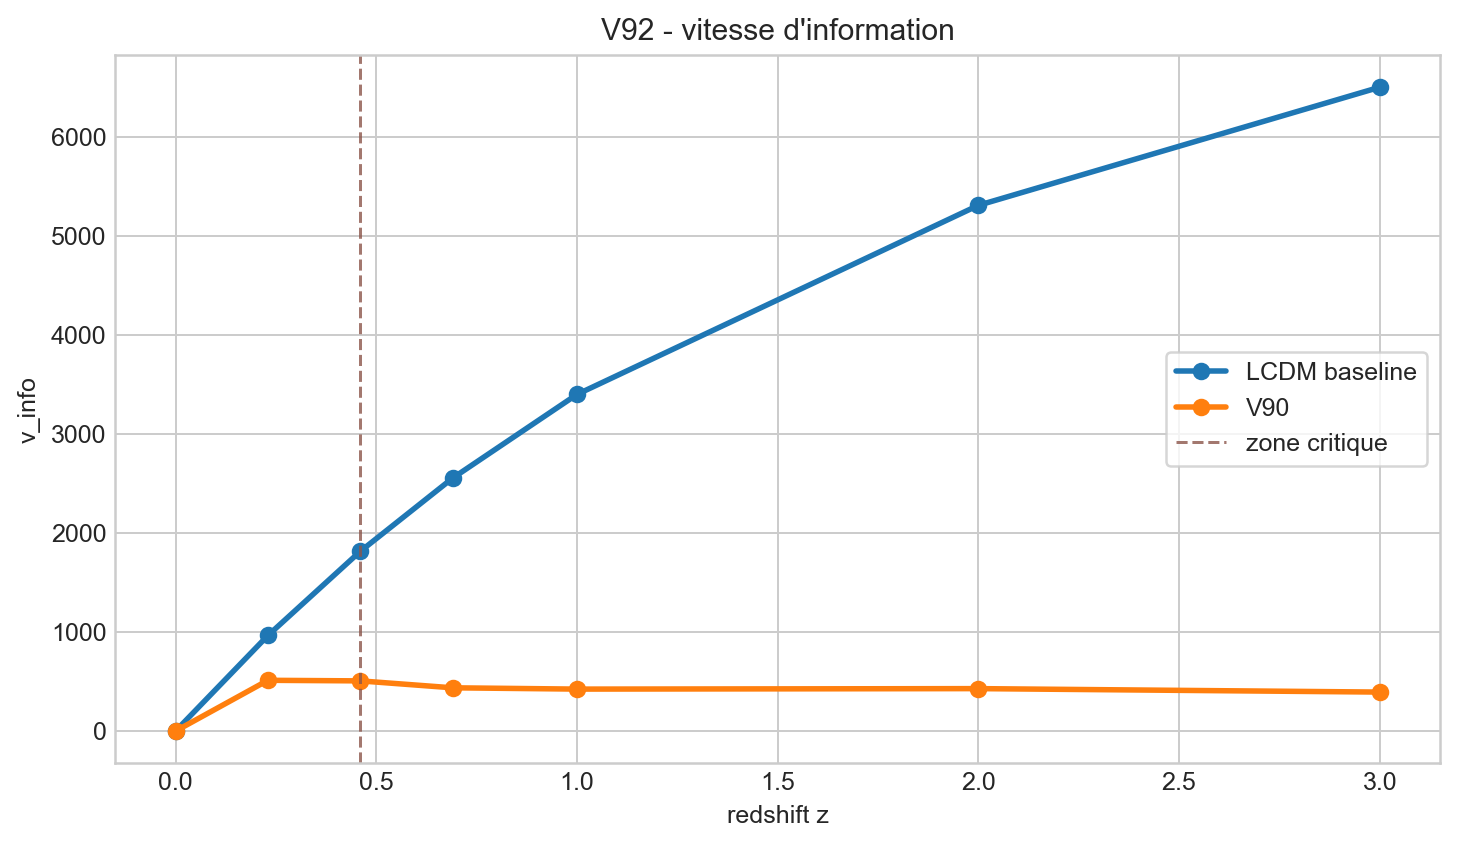
\includegraphics[width=0.92\linewidth]{v92_vinfo_comparison.png}
\caption{Comparaison de $v_{\mathrm{info}}(z)$ entre V90 et $\Lambda$CDM.}
\end{figure}

\subsection{Figure 2: ratios V90 / $\Lambda$CDM}
La seconde figure montre les ratios $d_{V90}/d_{\Lambda\mathrm{CDM}}$ et $v_{\mathrm{info},V90}/v_{\mathrm{info},\Lambda\mathrm{CDM}}$. Elle synthétise l'effet combiné du ralentissement du temps propre et de la compression géométrique.

\begin{figure}[htbp]
\centering
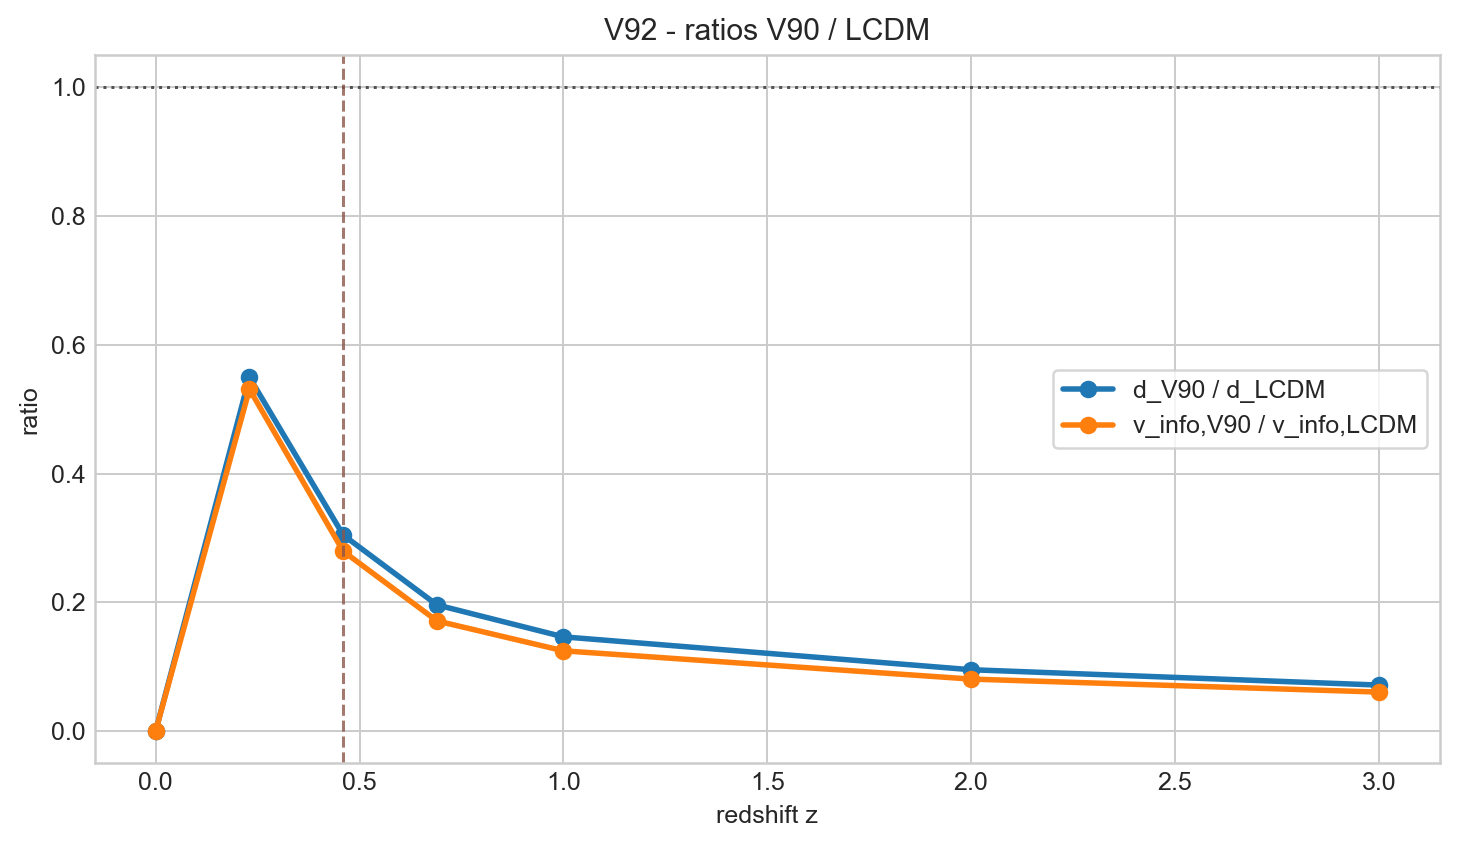
\includegraphics[width=0.92\linewidth]{v92_ratio_comparison.png}
\caption{Ratios de comparaison V90 / $\Lambda$CDM.}
\end{figure}

\subsection{Lecture scientifique}
Le message de V92 est simple: la zone critique ne se contente pas de modifier un paramètre global, elle produit un profil local sur $v_{\mathrm{info}}(z)$ et sur les ratios de distance. On voit ainsi trois effets distincts: le temps propre croît avec $z$, la vitesse d'information relative chute au voisinage de $z\approx0.46$, et les ratios V90 / $\Lambda$CDM restent inférieurs à 1 sur toute la grille testée. Cette lecture reste toutefois interne au modèle effectif et doit être confrontée à des données publiques pour devenir une affirmation physique.

\subsection{Résumé}
V92 est donc la version d'article de V91: même logique calculatoire, mais avec des graphes et un langage de lecture directement exploitable dans le manuscrit principal.

\begin{thebibliography}{9}
\bibitem{v50} Protocole V50 -- Détection du mécanisme d'intrication manquant via le scan $\gamma \to f\sigma_8(z)$, Mai 2026.
\bibitem{v51} Protocole V51 -- Potentiel complet avec intrication, Mai 2026.
\bibitem{v52} Protocole V52 -- Validation multi-secteur et préparation publication, Mai 2026.
\bibitem{v60} Protocole V60 -- Run du modèle complet + comparatif données, Mai 2026.
\bibitem{v61} Protocole V61 -- Analyse des résultats du testeur, Mai 2026.
\bibitem{v90} Protocole V90 -- Dynamique temps / vitesse / information / géométrie, Mai 2026.
\bibitem{v91} Protocole V91 -- Confrontation explicite V90 / $\Lambda$CDM et calibration locale, Mai 2026.
\bibitem{v92} Protocole V92 -- Figures comparatives V90 / $\Lambda$CDM et lecture article, Mai 2026.
\end{thebibliography}

\end{document}